\section{Current Experimental Measurements}\label{sec:current}
Several experimental groups are currently investigating transition form factors in the time-like regime, including, but not limited to;
\begin{itemize}
	\item TRIUMF $\pi^0 \to \epem \gamma$~\cite{FARZ} 
	\item A2 Collaboration $\eta \to \epem \gamma$~\cite{Berg,A2} 
	\item Multiple Groups $\omega\to\pi^0 \mu^+\mu^-$ ~\cite{Dzhelyadin:1980tj,Arnaldi:2009aa,Uras:2011zz}
	\item CLEO Collaboration $\eta'\to e^+e^-\gamma $~\cite{CLEO}
	\item Lepton-G $\eta'\to \mu^+\mu^-\gamma $~\cite{DZH}
	\item BESIII Collaboration $\eta'\to e^+e^-\gamma $~\cite{Ablikim:2015wnx}
	\item KLOE Collaboration $\phiDalT$~\cite{Babusci:2014ldz} .
\end{itemize}
The branching ratio of \etaPDal \ remained an upper limit, Fig.~\ref{fig:past}, until the BESIII collaboration finally measured it using 1.31 billion $J/\psi \to \gamma \etaP \to \gamma \gamma \epem$. From the BESIII data sample, Fig.~\ref{fig:past}, only 894 \etaPDal \ events were recorded which lead to a determination of the branching ratio $\Gamma_{\eta^{\prime} \rightarrow e^+e^- \gamma}  = 4.69 \pm 0.2 (\mathrm{stat.})\cdot 10^{-4}$ and a slope parameter, Eq.~\ref{eq:tffslope}, $b = 1.60\pm0.17(\mathrm{stat.})$ which is consistent with the measurement from Lepton-G ($1.7 \pm 0.4 (\mathrm{stat.})$). The slope parameter measured by BESIII and Lepton-G, which is the essential measurement needed for the HLbl contribution, is not sufficient to distinguish between different theoretical approaches listed in Tab.~\ref{tab:theory}. Some of the obstacles for not measuring the \etaPDal \ was the low branching ratio, pion contamination and low electron PID efficiency. These obstacles will be mitigated with CLAS12 by the high luminosity and excellent dilepton identification.

%The experiential results of the $\pi^0$ and $\omega$ present a puzzle because for the $\pi^0$ the measurement in the time-like region does not have agreement between several experiemtn
%
%The experimental results on the conversion decay of the $\omega$ meson, $\omega\to\pi^0 \mu^+\mu^-$  present a puzzle ~\cite{Dzhelyadin:1980tj,Arnaldi:2009aa,Uras:2011zz}. 
%The measurements suggest a dramatic increase of the transition form factor for large momentum transfers that is not consistent with VMD models nor explicable with modern theoretical advances. 
%These experimental results are in contradiction to measurements in the space-like regime~\cite{Achasov:2013btb}. 
%The situation makes it important to investigate the conversion decays of vector mesons. 
%
%{\it ... mention A2 measurement ? ...}
%
%The conversion decays of the  $\omega$ meson are currently being studied within the LMD group using data from the CLAS g12 experiment. 
%We plan to approach the conversion decays of the $\phi$ meson by analyzing the decay $\phi\to\eta\gamma^\star$ based on the proposed experiment. 
%The decay $\phi \to \pi^0\gamma^\star$ would enable access to higher dilepton masses and more precise mapping of transition form factors in this kinematic regime. However, the decay is OZI suppressed and statistically significant results may be obtained after a luminosity upgrade of the experiment facility.
%Current measurements by the KLOE collaboration for $\phi\to\eta e^+e^-$~\cite{Babusci:2014ldz} and $\phi\to\pi^0 e^+e^-$~\cite{Anastasi:2016bfh} have improved the values for the respective branching ratios by the SND and CMD-2 collaborations ~\cite{Achasov:2000ne,Akhmetshin:2000bw,Achasov:2002hs,Akhmetshin:2000wi}. The $\phi\to\eta e^+e^-$ measurement by KLOE is based on ~31000 events and deduces a slope parameter of $ \text{KLOE} \ b_{\phi\eta}=1.28\pm 0.10^{+0.09}_{-0.08} $.
%
%{\it ... figure of KLOE phi-eta TFF here? ...}
\begin{figure}[h!]\begin{center}
		\subfloat[$\phi$ Dalitz and conversion spectra from g12][]{ %Feynman diagram of $\etaP$ Dalitz decay
			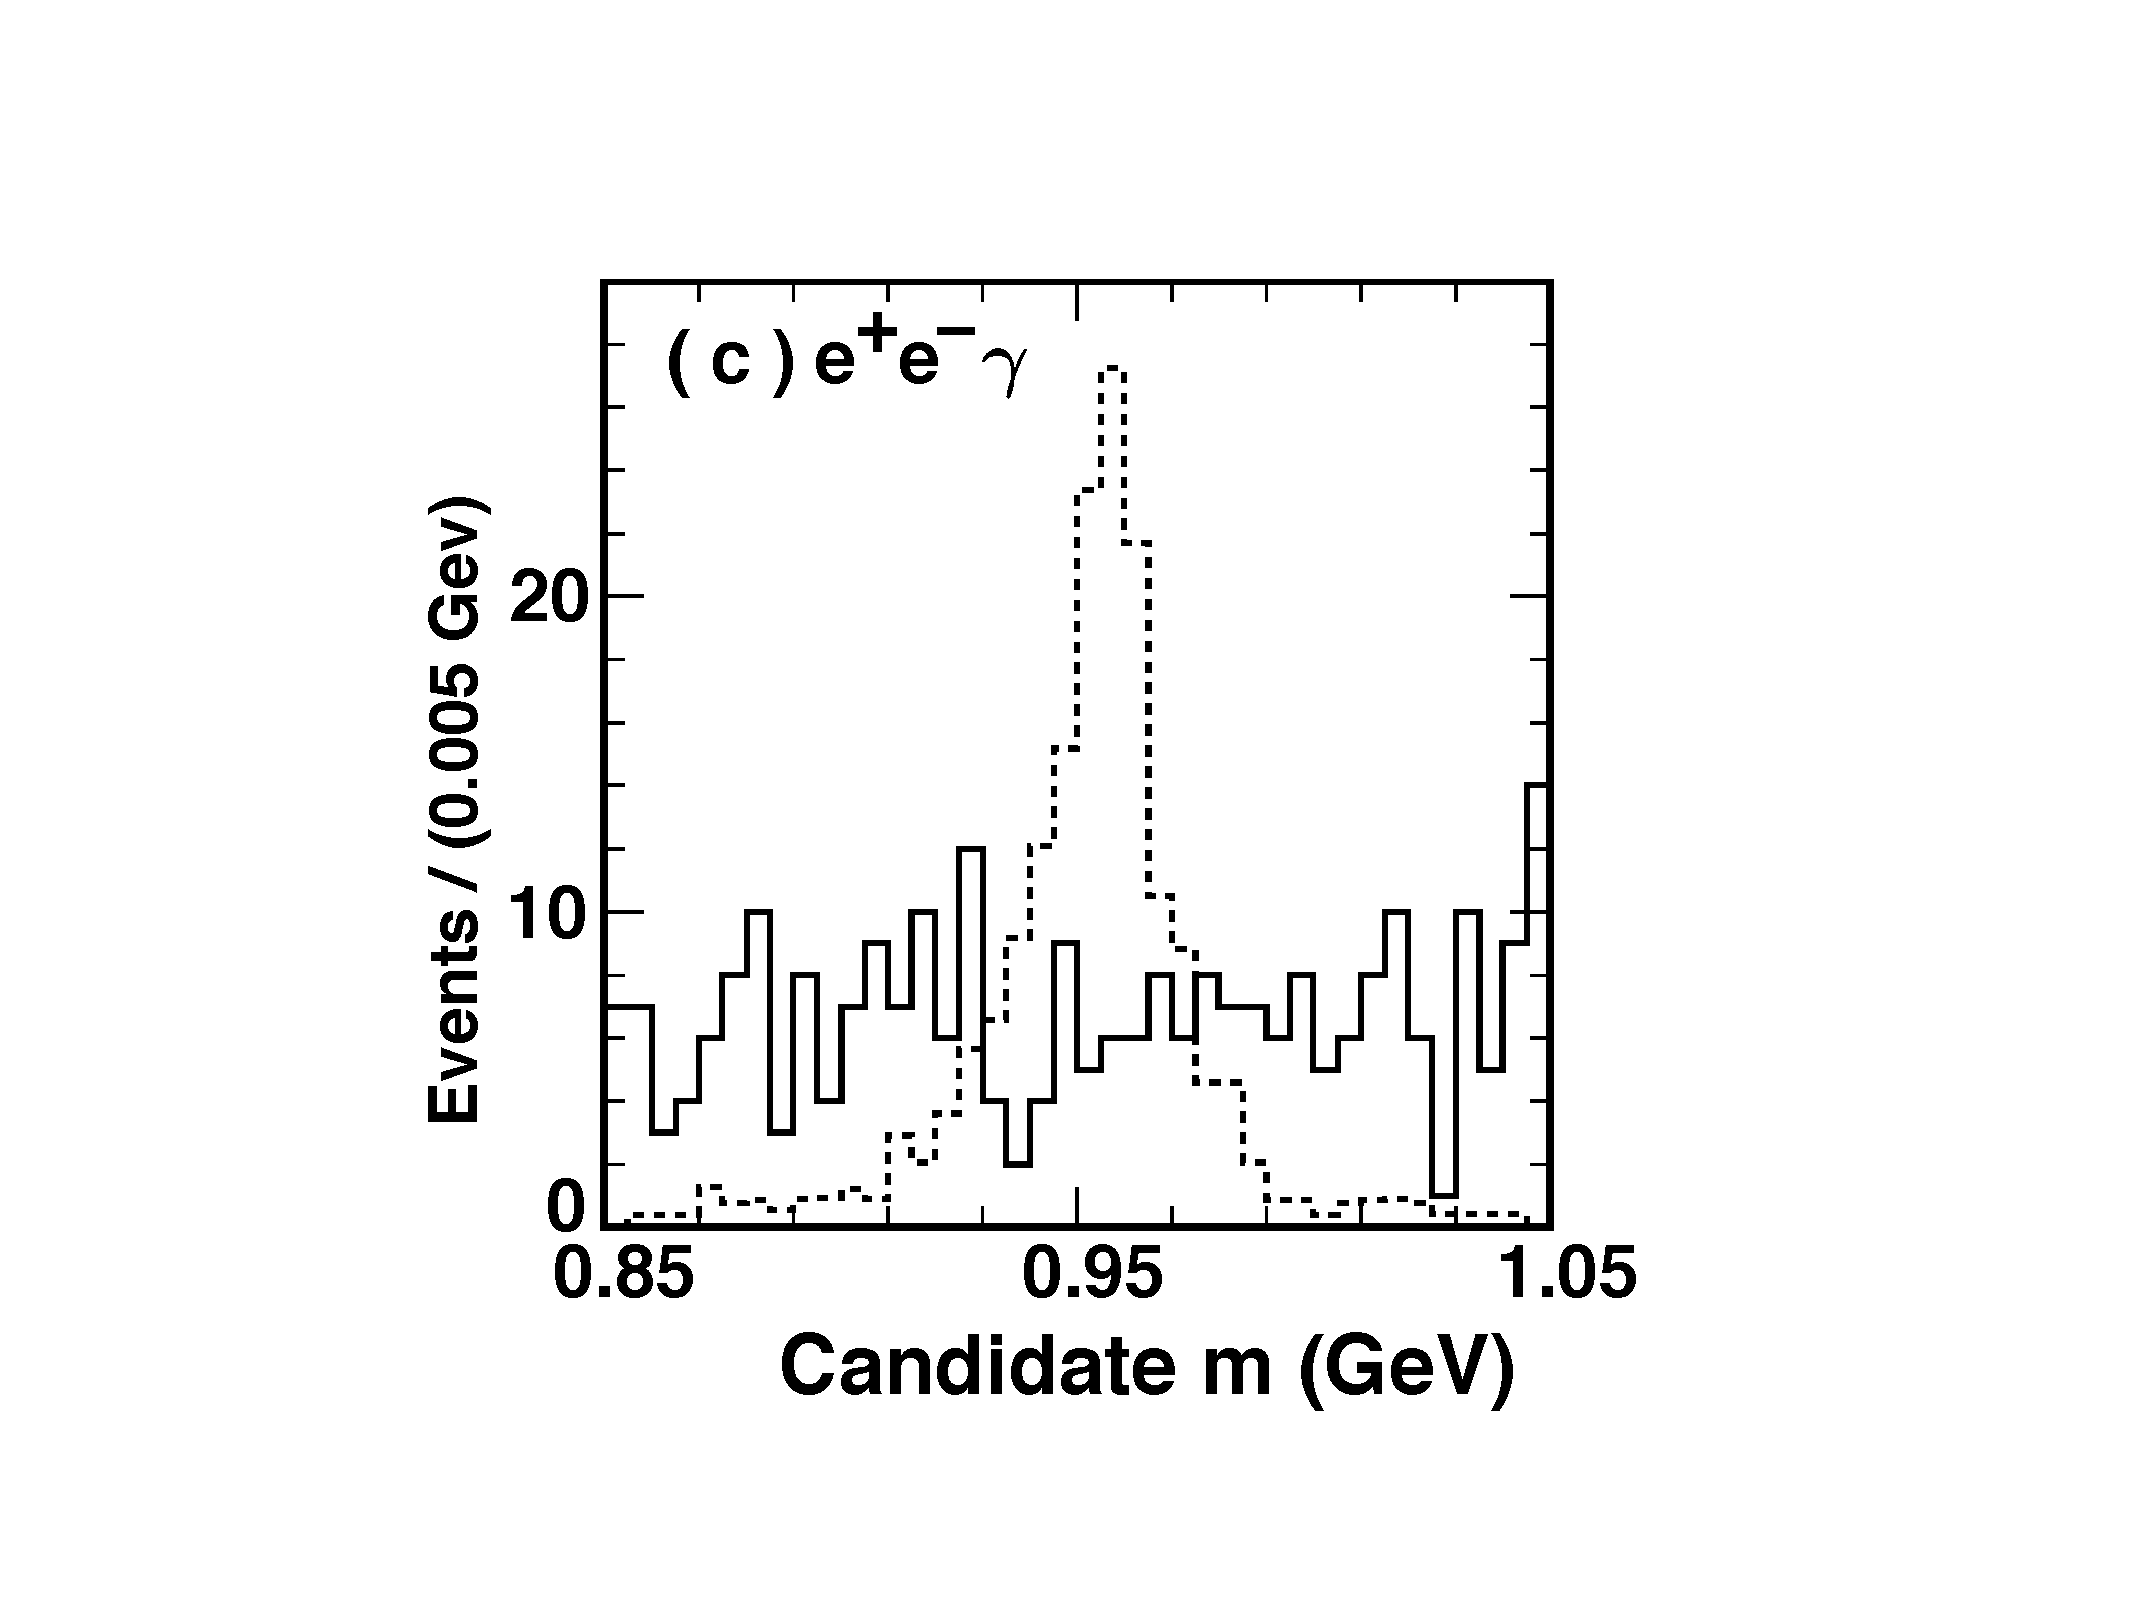
\includegraphics[width=1.0\columnwidth,height=1.0\qfigheight]{\grpath/current_status/CLEO_keynote.pdf}\label{fig:CLEO}
		}
		\\
		\subfloat[$\etaP$ Dalitz and conversion spectra from BESIII][]{ %Feynman diagram of $\etaP$ two photon decay
			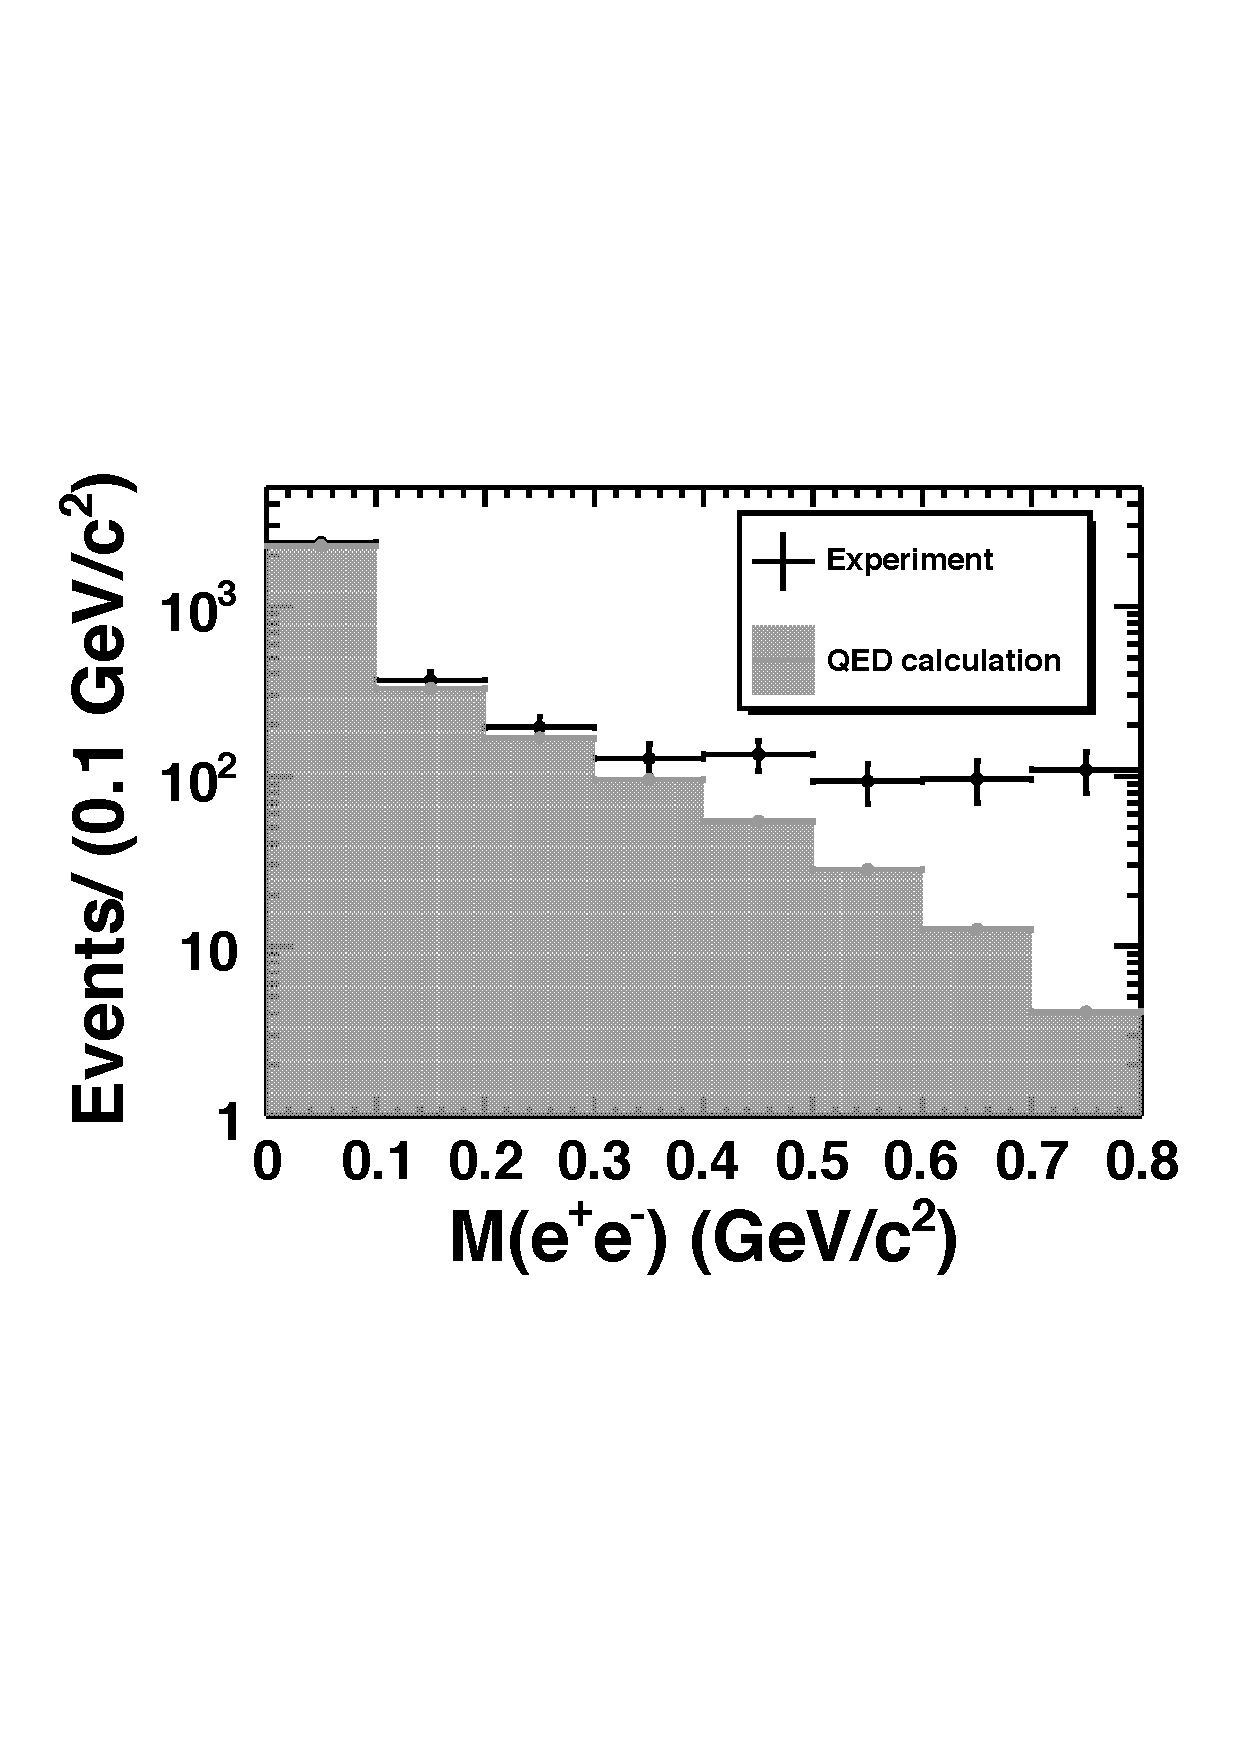
\includegraphics[width=0.8\columnwidth,height=1.8\qfigheight]{\grpath/current_status/BESIII_EtaP.pdf}\label{fig:BESIII}
		}
		\caption[Counts rates for \etaTP from previous experiements]{\label{fig:past} ~\subref{fig:CLEO} Missing mass off of the proton for \etaPDal \ from the CLEO collaboration~\cite{CLEO}, solid line(data), dashed(MC expectation).~\subref{fig:BESIII}Counts of $M(\epem)$ from the first published observation of the \etaPDal \  by BESIII~\cite{BESIII}. }
\end{center}\end{figure}
	\FloatBarrier 	
	\subsection{Previous CLAS analyses}
	The LMD (Light Meson Decay) group of CLAS was established to investigate the decay properties of light mesons. Two experiments in CLAS are currently being analyzed in the LMD group. The g12 experiment, performed with CLAS, is one experiment chosen due to its ability to identify leptons with the use of the Cherenkov detectors (CC).
	% performed with the g12 experiment
	The g12 experiment produced a data set of photon-induced reactions. Fortunately, the Cherenkov Counters were filled with perflourbutane ($C_4F_{10}$) and a trigger consisting of a coincidence between the (ST$\cdot$TOF)(CC$\cdot$EC), allowing the study of dilepton reactions throughout the entire beam energy range $1.15 \ \mathrm{GeV}<E_\gamma <5.45 \ \mathrm{GeV}$. The g12 experiment ran for 44 days however, the trigger that allowed for \epemT identification was established for $\sim$29 days of beam-time. Using approved dilepton identification~\cite{g12note}, preliminary analyses of g12 involving dileptons include the decays:
	\begin{itemize}
		\item $\Delta \to p \epem$ (Transition form factor)
		\item $\eta \to \epem \gamma$ (Transition form factor)
	\end{itemize}
	while advanced analyses involving dileptons include:
	\begin{itemize}
		\item $\piz \to \epem \gamma$ (Differential Cross-Section)
		\item $\omega / \rho \to \epem$ (Interference of $\omega/\rho$ )
		\item $\omega \to \epem \piz$ (Transition form factor)
		\item $\etaP \to \epem \gamma$ (Transition form factor / branching ratio)
	\end{itemize}
	The g12 \etaPDal \ analysis provided CLAS its first look at the possibility of measuring the branching ratio and transition form factor. 
	\subsubsection{G12 Lepton and Neutral Trigger Setup}\label{sec.data.trig.lepton}
In g12, since the CC was filled with gas, it was possible to include the CC as a component of the trigger. 
There were three trigger ``bits'' used for lepton identification in g12 as listed in Tab.~\ref{tab:data.trig.conf.2}. Each ``bit'' used a (EC$\cdot$CC) configuration to identify leptons. The (EC$\cdot$CC) configuration required a coincidence between the electromagnetic calorimeter and the Cherenkov subsystems. This coincidence was established by using the voltage sum of the CC for a sector and the voltage sum of the EC for the same sector and comparing each sum to a preset threshold described in Tab.~\ref{tab:data.ecccthresh}. The EC voltage sum threshold comparison is done on both the EC$_\mathrm{inner}$ and EC$_{\mathrm{total}}$ which are the EC voltage signals for the energy deposited in the inner layer and in all layers. The labels of photon or electron specified in Tab.~\ref{tab:data.ecccthresh} are not actual photons or electrons, but were considered a first-order approximation for detection. The particle identification is done at the analysis level. The method for determining the (EC$\cdot$CC) does not allow for multiple lepton triggering in the same sector. Determining multiple leptons in the same sector is done at the analysis level. 

The ``bit 6'' trigger configuration, (ST$\cdot$TOF)$\cdot$(EC$\cdot$CC) requires a Start-Counter (ST) and Time-of-Flight (TOF) coincidence along with a coincidence between the electromagnetic calorimeter and the Cherenkov subsystems described above. The (ST$\cdot$TOF) configuration of ``bit 6'' did not have to be in the same sector as the (EC$\cdot$CC) configuration of ``bit 6''. The ``bit 11'' trigger configuration, (EC$\cdot$CC)$\times$2 requires two coincidences between the electromagnetic calorimeter and the Cherenkov subsystems described above, in two different sectors. 

The ``bit 5'' trigger configuration was also established as a lepton trigger. It required EC hits in two sectors. The ``bit 5'' trigger configuration was also established to analyze physics involving two or more neutral particles accompanied with a charged track, such as exclusive \pizT \ production in which the \pizT \ decays via 2 photons. The method for ``bit 5'' voltage sum comparison is identical to the EC voltage sum of ``bit 6'' and ``bit 11''

It should be noted that none of the lepton triggers required a MOR signal, allowing for physics involving leptons to be measured starting from g12's lowest tagger detection value of 1.142~GeV.

%\begin{table}
\begin{minipage}{\textwidth}
\begin{center}


\caption[Trigger Configuration 1]{\label{tab:data.trig.conf.1}Trigger configuration for \g12 runs from 56363 to 56594 and 56608 to 56647. (\abbr{ST}$\cdot$\abbr{TOF})$_{i}$ indicates a trigger-level track defined as a coincidence between a start counter and time-of-flight hit in the \ith\ sector. \abbr{MORA} and \abbr{MORB} represent coincidences with tagger hits within a certain energy range as specified in Table~\ref{tab:data.trig.mor}.}

\begin{tabular}{cccc}

\hline

\multicolumn{4}{c}{\g12 runs 56363--56594, 56608--56647} \\

\hline

bit & definition & L2 multiplicity & prescale \\

\hline

1 & \abbr{MORA}$\cdot$(\abbr{ST}$\cdot$\abbr{TOF})$_{1}\cdot$(\abbr{ST}$\cdot$\abbr{TOF})$_{i\neq 1}$ & -- & 1 \\
2 & \abbr{MORA}$\cdot$(\abbr{ST}$\cdot$\abbr{TOF})$_{2}\cdot$(\abbr{ST}$\cdot$\abbr{TOF})$_{i\neq 2}$ & -- & 1 \\
3 & \abbr{MORA}$\cdot$(\abbr{ST}$\cdot$\abbr{TOF})$_{3}\cdot$(\abbr{ST}$\cdot$\abbr{TOF})$_{i\neq 3}$ & -- & 1 \\
4 & \abbr{MORA}$\cdot$(\abbr{ST}$\cdot$\abbr{TOF})$_{4}\cdot$(\abbr{ST}$\cdot$\abbr{TOF})$_{i\neq 4}$ & -- & 1 \\
5 & \abbr{MORA}$\cdot$(\abbr{ST}$\cdot$\abbr{TOF})$_{5}\cdot$(\abbr{ST}$\cdot$\abbr{TOF})$_{i\neq 5}$ & -- & 1 \\
6 & \abbr{MORA}$\cdot$(\abbr{ST}$\cdot$\abbr{TOF})$_{6}\cdot$(\abbr{ST}$\cdot$\abbr{TOF})$_{i\neq 6}$ & -- & 1 \\
7 & \abbr{ST}$\cdot$\abbr{TOF} & -- & 1 \\
8 & \abbr{MORA}$\cdot$(\abbr{ST}$\cdot$\abbr{TOF})$\times$2 & -- & 1 \\
11\footnote{bit 11 and \abbr{MORB} were included in the trigger starting with run 56519.} & \abbr{MORB}$\cdot$(\abbr{ST}$\cdot$\abbr{TOF})$\times$2 & -- & 1 \\
12 & (\abbr{ST}$\cdot$\abbr{TOF})$\times$3 & -- & 1 \\

\hline \hline

\end{tabular}


\end{center}
\end{minipage}
\end{table}
\vspace{20pt}
 % label: tab:data.trig.conf.1

\begin{table}
\begin{minipage}{\textwidth}
\begin{center}


\caption[Trigger Configuration 2]{\label{tab:data.trig.conf.2}Trigger configuration for g12 runs from 56595 to 56607 and 56648 to 57323. \vspace{0.75mm}}

\begin{tabular}{cccc}

\hline

\multicolumn{4}{c}{g12 runs 56595--56607, 56648--57323 } \\

\hline

bit & definition & L2 multiplicity& prescale \\

\hline

1 & \abbr{MORA}$\cdot$(\abbr{ST}$\cdot$\abbr{TOF}) & 1 & 1000/300\\
2 & \abbr{MORA}$\cdot$(\abbr{ST}$\cdot$\abbr{TOF})$\times$2 & 2/-- & 1 \\
3 & \abbr{MORB}$\cdot$(\abbr{ST}$\cdot$\abbr{TOF})$\times$2 & 2 & 1 \\
4 & \abbr{ST}$\cdot$\abbr{TOF} & 1 & 1000/300 \\
5 & (\abbr{ST}$\cdot$\abbr{TOF})$\cdot$\abbr{EC}$\times$2 & 1 & 1 \\
6 & (\abbr{ST}$\cdot$\abbr{TOF})$\cdot$(\abbr{EC}$\cdot$\abbr{CC}) & 2 & 1 \\
7 & \abbr{MORA}$\cdot$(\abbr{ST}$\cdot$\abbr{TOF})$\cdot$(\abbr{EC}$\cdot$\abbr{CC}) & -- & 1 \\
8 & \abbr{MORA}$\cdot$(\abbr{ST}$\cdot$\abbr{TOF})$\times$2 & -- & 1 \\
11 & (\abbr{EC}$\cdot$\abbr{CC})$\times$2 & -- & 1 \\
12 & (\abbr{ST}$\cdot$\abbr{TOF})$\times$3 & -- & 1 \\

\hline \hline

\end{tabular}


\end{center}
\end{minipage}
\end{table}
\vspace{20pt}
 % label: tab:data.trig.conf.2

%\begin{table}
\begin{minipage}{\textwidth}
\begin{center}


\caption[Trigger Configuration for Single-sector Runs]{\label{tab:data.trig.conf.3}Trigger configuration for the single-prong runs of \g12. Trigger bits 7--12 were not used for these runs. \vspace{0.75mm}}

\begin{tabular}{cccc}

\hline

bit & definition & L2 multiplicity & prescale \\

\hline

1 & \abbr{MORA}$\cdot$(\abbr{ST}$\cdot$\abbr{TOF})$_{1}$ & sector 1 & 1 \\
2 & \abbr{MORA}$\cdot$(\abbr{ST}$\cdot$\abbr{TOF})$_{2}$ & sector 2 & 1 \\
3 & \abbr{MORA}$\cdot$(\abbr{ST}$\cdot$\abbr{TOF})$_{3}$ & sector 3 & 1 \\
4 & \abbr{MORA}$\cdot$(\abbr{ST}$\cdot$\abbr{TOF})$_{4}$ & sector 4 & 1 \\
5 & \abbr{MORA}$\cdot$(\abbr{ST}$\cdot$\abbr{TOF})$_{5}$ & sector 5 & 1 \\
6 & \abbr{MORA}$\cdot$(\abbr{ST}$\cdot$\abbr{TOF})$_{6}$ & sector 6 & 1 \\

\hline \hline

\end{tabular}


\end{center}
\end{minipage}
\end{table}
\vspace{20pt}
 % label: tab:data.trig.conf.3

%\begin{table}
\begin{center}


\caption[Trigger Configuration (Tagger)]{\label{tab:data.trig.mor}Master-\abbr{OR} definitions for \g12. The \abbr{TDC} counters were used in the trigger and since each of these corresponds to several energy paddles, the energies given here are approximate. $T$-counter number 1 corresponds to the highest energy photon of approximately 5.4~GeV. Both \abbr{MORA} and \abbr{MORB} are referenced in terms of the trigger logic in Tables~\ref{tab:data.trig.conf.1}, \ref{tab:data.trig.conf.2} and \ref{tab:data.trig.conf.3}. The single-prong runs are listed in Table~\ref{tab:data.cook.singlesecruns}.\vspace{0.75mm}}

\begin{tabular}{c|cc|cc}

\hline

          & \multicolumn{2}{c|}{\abbr{MORA}} & \multicolumn{2}{c}{\abbr{MORB}} \\
run range & $T$-counters & energy (GeV)     & $T$-counters & energy (GeV) \\

\hline

56363--56400 & 1--47 & 1.7--5.4 & -- & -- \\
56401--56518 & 1--25 & 3.6--5.4 & -- & -- \\
56519--57323 & 1--19 & 4.4--5.4 & 20--25 & 3.6--4.4 \\

\hline

\emph{single-sector} & 1--31 & 3.0--5.4 & -- & -- \\

\hline \hline

\end{tabular}


\end{center}
\end{table}
\vspace{20pt} % label:  tab:data.trig.mor

\begin{table}
\begin{center}


\caption[\abbr{EC} and \abbr{CC} Trigger Thresholds]{\label{tab:data.ecccthresh}Threshold values for the electromagnetic calorimeter (\abbr{EC}) and Cherenkov counter (\abbr{CC}) during the g12 running period. \abbr{EC} thresholds are shown as \emph{inner}/\emph{total}, and \abbr{CC} thresholds are shown as \emph{left}/\emph{right}.\vspace{0.75mm}}

\begin{tabular}{cc|c}
\hline

\multicolumn{2}{c|}{\abbr{EC}} & \abbr{CC} \\

\emph{``photon"} & \emph{``electron"} \\


\hline

50/100~mV & 60/80~mV & 20/20~mV \\
150/300~MeV & 180/240~MeV & $\sim$0.4~photo-electrons \\

\hline \hline

\end{tabular}
\end{center}
\end{table}
\vspace{20pt} % label: tab:data.ecccthresh
\FloatBarrier
	\subsubsection{G12 Detection of \epemT Events} 
     The g12 experiment derived a set of conditions for identifying electron/positrons pairs in CLAS by employing specific cuts to the number of photo-electrons (NPE) detected in the CC, a match in azimuthal angle $\phi$ from a charged track in the Drift Chambers (DC) to the $\phi$ of the CC, as well as comparing the momentum of the charged track to the energy deposited in the EC. These cuts can be found in Tab.~\ref{tab:ISLEP_cuts}.
	\begin{table}[htpb]
\begin{minipage}{\textwidth}
\begin{center}


\caption[Electron/Positron PID Cuts]{\label{tab:ISLEP_cuts}Cuts applied to the \emph{CC} and \emph{EC} to perform electron/positron \emph{PID}. Table source:~\cite{thesiskunkel} \vspace{0.75mm}}

\begin{tabular}{c|c|c}

\hline
Subsystem & Quantity & Cut \\
\hline
\multirow{2}{*}{\emph{CC}}  & \# of photo-electrons (\emph{NPE})  & \emph{NPE} $>$ 2.5 \\
 &  \emph{DC} $\phi$ \& \emph{CC} $\phi$  & \emph{DC} $\phi$ = \emph{CC} $\phi$ \\
\hline
\multirow{2}{*}{\emph{EC}}  & q$^{\pm}$ momentum threshold (p$\mathrm{_{thres}}$) & \multirow{2}{*}{p$\mathrm{_{thres}^{high}} < \ $E$\mathrm{_{calo}} <$ p$\mathrm{_{thres}^{low}}$ } \\
&  \& \emph{EC} deposited energy (E$\mathrm{_{calo}}$) & \\
\hline \hline
\end{tabular}

\end{center}
\end{minipage}
\end{table}

	To validate the g12 electron/positron PID, a comparison of  the CC and EC quantities was performed for all charged tracks CC/EC hit signatures and while selecting events from $\pi^0$ decay. To separate the $\pi^0$ events from the $\pi^+\pi^-$ events, all charged pions were assigned the mass of electrons and cuts were placed on the missing energy of $\gamma p \rightarrow p e^+ e^-$ as well as a cut on the missing mass squared of $\gamma p \rightarrow p$, values found in Tab.~\ref{tab:lep_cuts}. A graphical depiction of the cuts applied to separate $\pi^0$ events from the $\pi^+\pi^-$ events is seen in Fig.~\ref{fig:islep.cuts}.
	\begin{table}[htpb]
\begin{minipage}{\textwidth}
\begin{center}


\caption[Cuts To Separate $\pi^0$ from $\pi^{+}\pi^{-}$ for \emph{PID} Validation]{\label{tab:lep_cuts}Cuts applied to separate $\pi^0$ events from $\pi^{+}\pi^{-}$ events. Table source:~\cite{thesiskunkel} \vspace{0.75mm}}

\begin{tabular}{c|c|c}

\hline
Cut Topology & Topology Quantity & Value  \\
\hline
$\gamma p \rightarrow p e^+ e^-$ & Missing Energy ($\mathrm{M_E}$) & $>0.075$~GeV \\
\hline
\multirow{2}{*}{$\gamma p \rightarrow p $}  & \multirow{2}{*}{Missing mass squared ($\mathrm{M_x^2}$)} & $<$ 0.0779~GeV$^2$ for $\pi^0$ events \\
&  & $>$ 0.0779~GeV$^2$ for $\pi^{+}\pi^{-}$ events\\
\hline \hline
\end{tabular}


\end{center}
\end{minipage}
\end{table}

	The values of the threshold momentum are calculated from empirical studies and are based upon calculations using the momentum obtained from the DC$p$ under the following criteria;
	\begin{align}
	\mathrm{p_{thres}^{low}} = \alpha p *(p+EC_{P\_LO})/p \nonumber \\
	\mathrm{p_{thres}^{high}} = \alpha p *(p+EC_{P\_HIGH})/p \nonumber
	\end{align}
	where $EC_{P\_LO} = -0.3$, $EC_{P\_HIGH} = 0.5$ and
	\begin{align}
	\alpha p =
	\begin{cases}
	.23*p + .071p^2 - .032p^3, & p<1.0 \text{~GeV} \\
	0.272p, & p>1.0 \text{~GeV} \\
	\end{cases}\nonumber
	\end{align}
	
	
\begin{figure}[h!]\begin{center}
			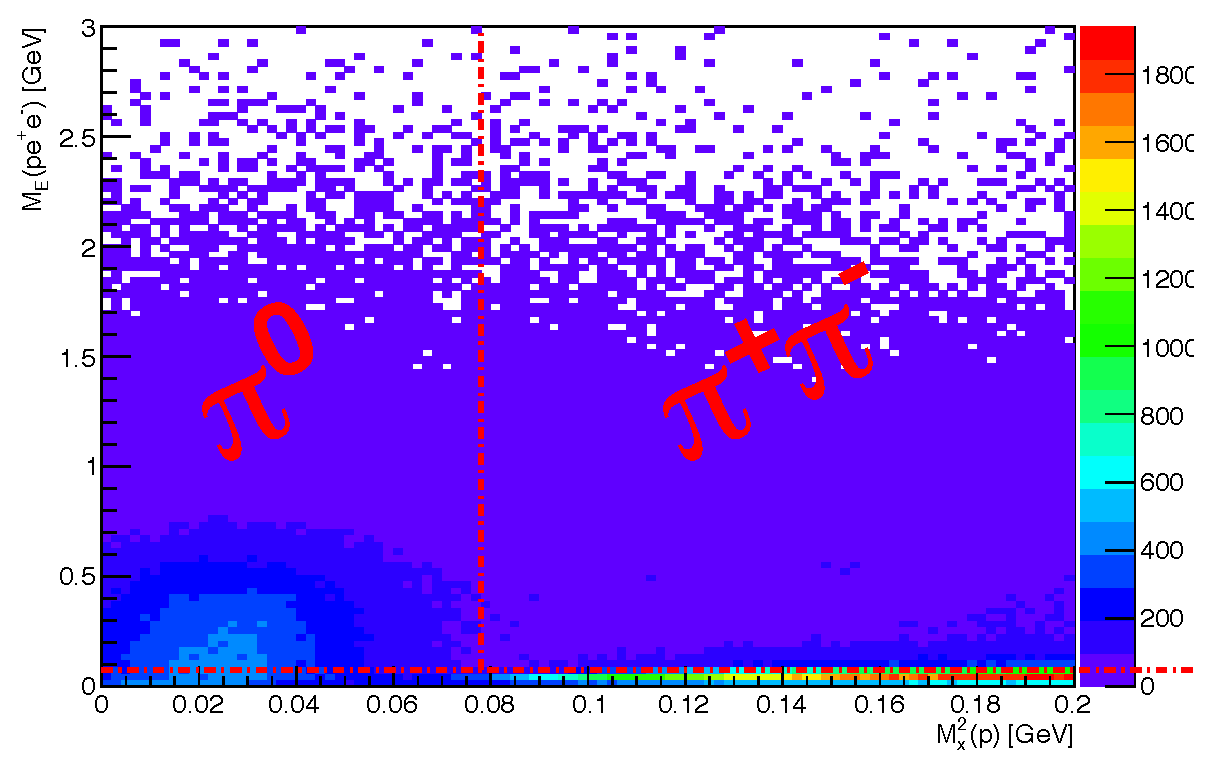
\includegraphics[width=0.8\figwidth]{\grpath/lepton/Lepfeature_cuts.eps}
			\caption[Cuts Applied to Isolate $\pi^0$ and $\pi^+\pi^-$ for PID Validation]{\label{fig:islep.cuts}Plot of missing mass squared of off proton (horizontal) vs. missing energy of proton $e^+e^-$ (vertical). The red dashed vertical line depicts the $\pi^+\pi^-$ threshold mass cut while the horizontal red dashed line represents the missing energy cut-off used to separate $\pi^+\pi^-$ from $\pi^0$. Image source:~\cite{thesiskunkel,g12note}}
\end{center}\end{figure}
%\begin{figure}[h!]\begin{center}
%		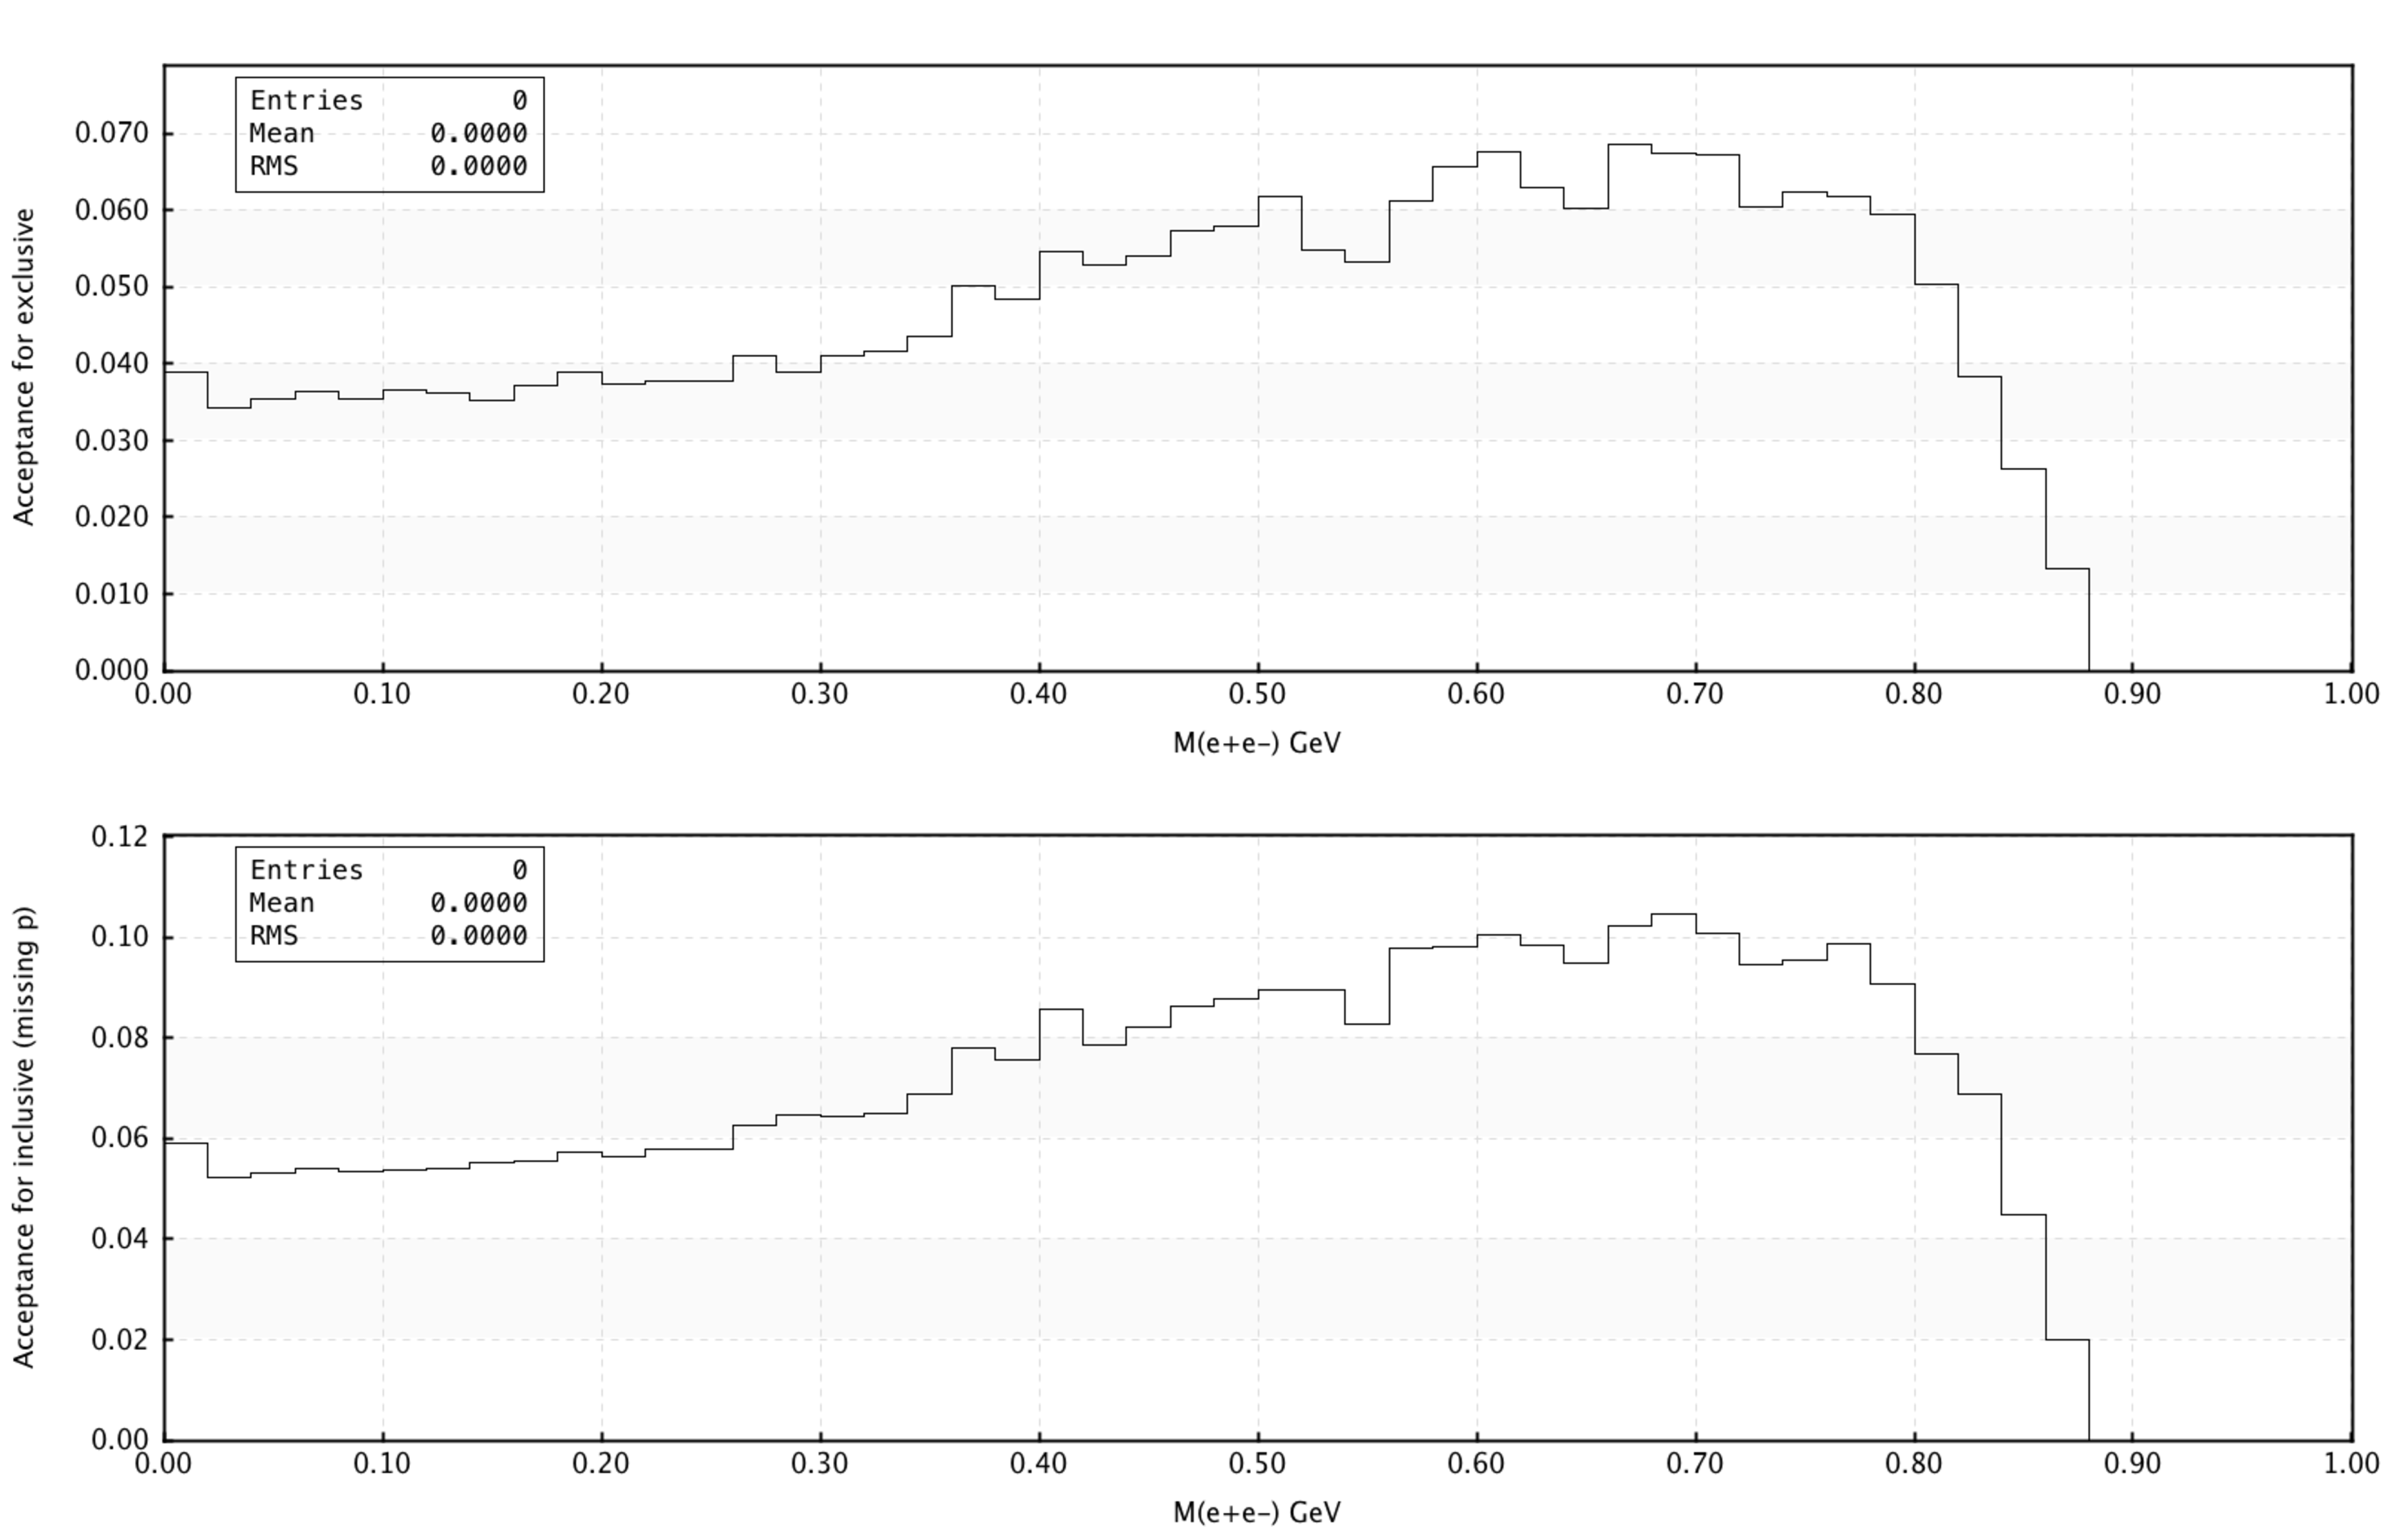
\includegraphics[width=\figwidth,height=1.2\qfigheight]{\grpath/counts/75_TORUS/VMD/VMD_Acceptance.pdf}
%		\caption[Acceptance, as a function of $M(\epem)$]{\label{fig:VMDaccepted}{Acceptance using a VMD decay model, as a function of $M(\epem)$ for the exclusive (Top) and inclusive reconstruction scheme(Bottom). }}
%	\end{center}\end{figure}		
\FloatBarrier
\paragraph{\label{sec:data.lepton.cc}CC Comparison}

The NPE measured by the CC for all positron/electron (e$^+$/e$^-$) candidates can be seen in Fig~\ref{fig:islep.CC}. The sharp decline prior to 2.5 NPE is due to photo-electrons created by electron/positrons, pions traveling through the CC or pions producing delta-electrons which pass through the CC. Delta-electrons are created as an effect of the ionization of gases that could be present when the pion travels through the DC. These types of electrons are typically lower in momentum than the electrons obtained from particle decays in CLAS and thus should emit less NPE per unit length.

Through mass conservation the particles for the $\pi^0$ events must be $e^+e^-$ pairs. In comparison to fig.~\ref{fig:islep.CC}, fig.~\ref{fig:islep.CC1} plots the NPE measured by the CC for all e$e^+e^-$ pairs for $\pi^0$ events selected as shown in fig.~\ref{fig:islep.cuts}. It can be seen that the sharp decline prior to NPE = 2.5 is reduced leaving mostly electrons or positrons signatures in the CC concluding that the g12 CC NPE cut is valid for identifying $e^+e^-$ pairs while rejecting $\pi^+\pi^-$ pairs.
Using the current cuts of NPE and hit angle, the suppression of di-leptons was sufficient without including additional cuts on the CC such as a timing comparison to the TOF.

%
\begin{figure}\begin{center}
		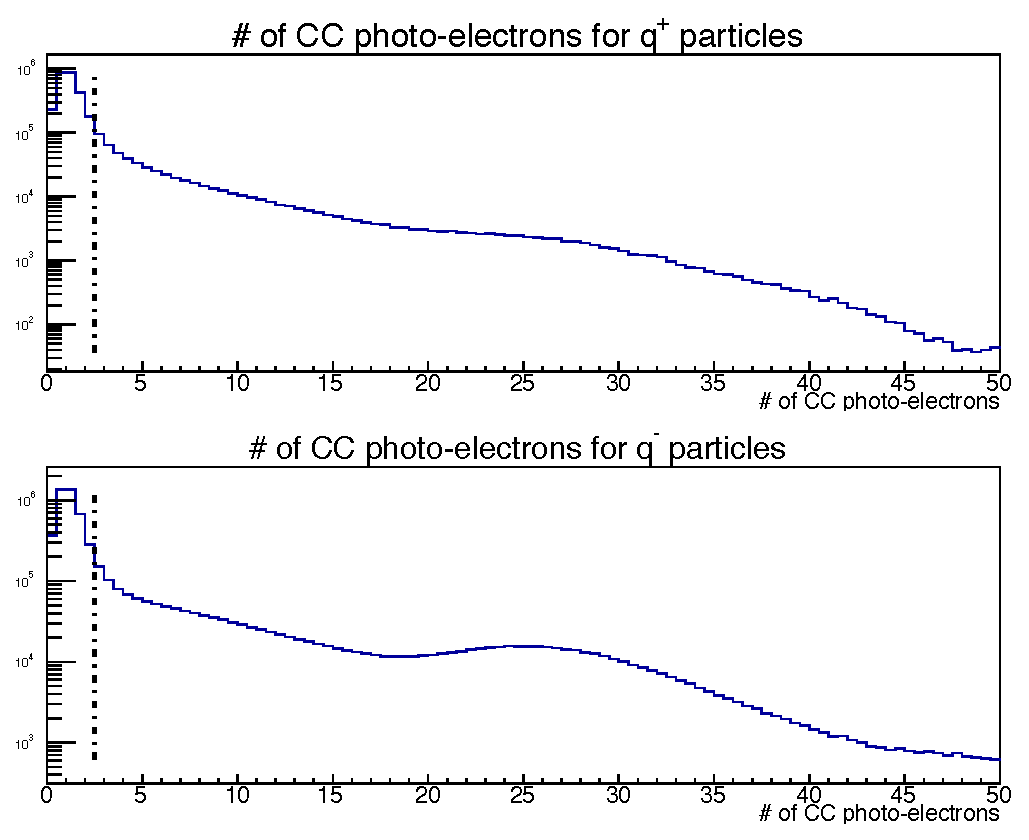
\includegraphics[width=0.8\figwidth]{figures/lepton/CC_nPE.eps}
		\caption[Number of Photo-electrons Measured by CC for All $e^-$ and $e^+$ Candidates]{\label{fig:islep.CC}Plot of NPE measured by CLAS CC subsystem for positron/electron candidates top/bottom respectively. The dashed dotted vertical line depicts the cut applied if using the g12 lepton PID scheme. Image source:~\cite{thesiskunkel}}
\end{center}\end{figure}
	
\begin{figure}\begin{center}
			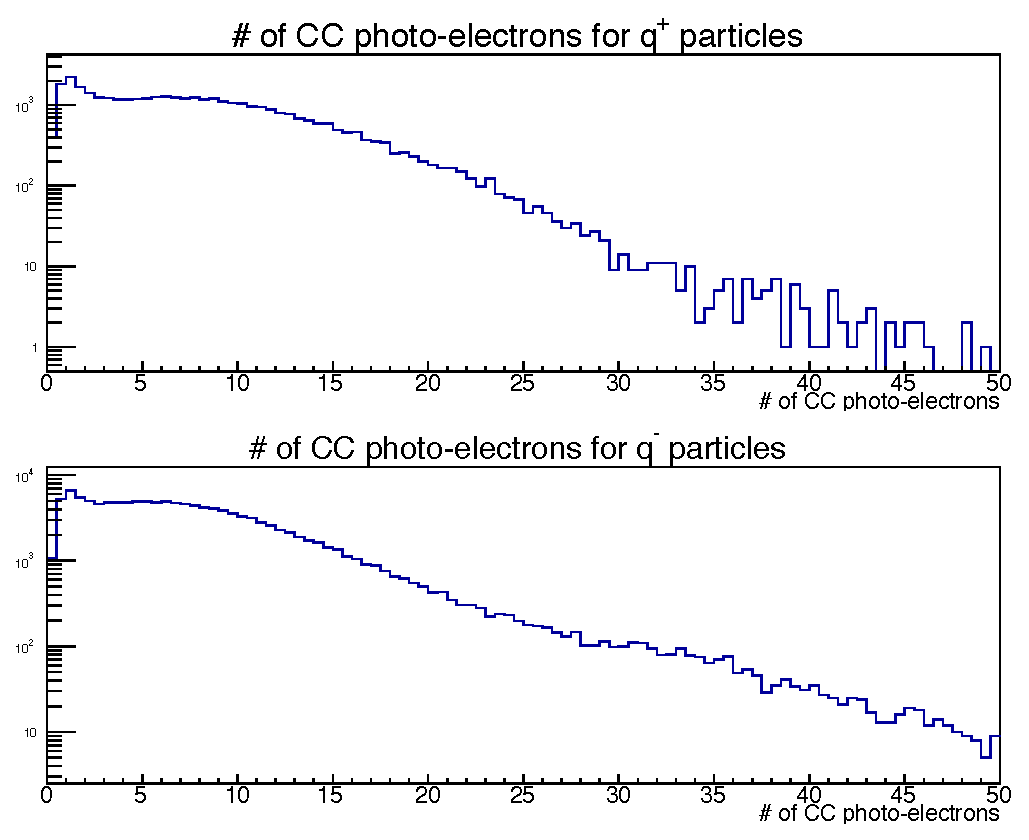
\includegraphics[width=0.8\figwidth]{figures/lepton/CC_NPEcut.eps}
			\caption[Number of Photo-electrons Measured by CC for $\pi^0$ Events]{\label{fig:islep.CC1}Plot of NPE measured by CLAS CC subsystem when selecting $\pi^0$ events seen in Fig~\ref{fig:islep.cuts}, positron/electron candidates top/bottom respectively. Image source:~\cite{thesiskunkel}}
\end{center}\end{figure}
		
\FloatBarrier

\paragraph{\label{sec:data.lepton.ec}EC Comparison}
		
		Similarly to the CC comparison, figures~\ref{fig:islep.pimEClow},~\ref{fig:islep.pimEChigh},~\ref{fig:islep.pipEClow},~\ref{fig:islep.pipEChigh} depict the  p$\mathrm{_{thres}^{low}}$ and  p$\mathrm{_{thres}^{low}}$ cuts listed in Tab.~\ref{tab:ISLEP_cuts} for the q$^-$ and q$^+$ tracks respectively. After $\pi^0$ event selection, seen in figures~\ref{fig:islep.pimEC},~\ref{fig:islep.pimECcut} ,~\ref{fig:islep.pipEC} ,~\ref{fig:islep.pipECcut}, the bulk of $e^+e^-$ events reside within the region of the cut acceptance therefore it is evident that the g12 EC cuts are valid for identifying \epemT \ pairs. The following four plots are for electron($e^-$) PID validation of the g12 EC cuts described in Tab.~\ref{tab:ISLEP_cuts}.
		%
\begin{figure}\begin{center}
				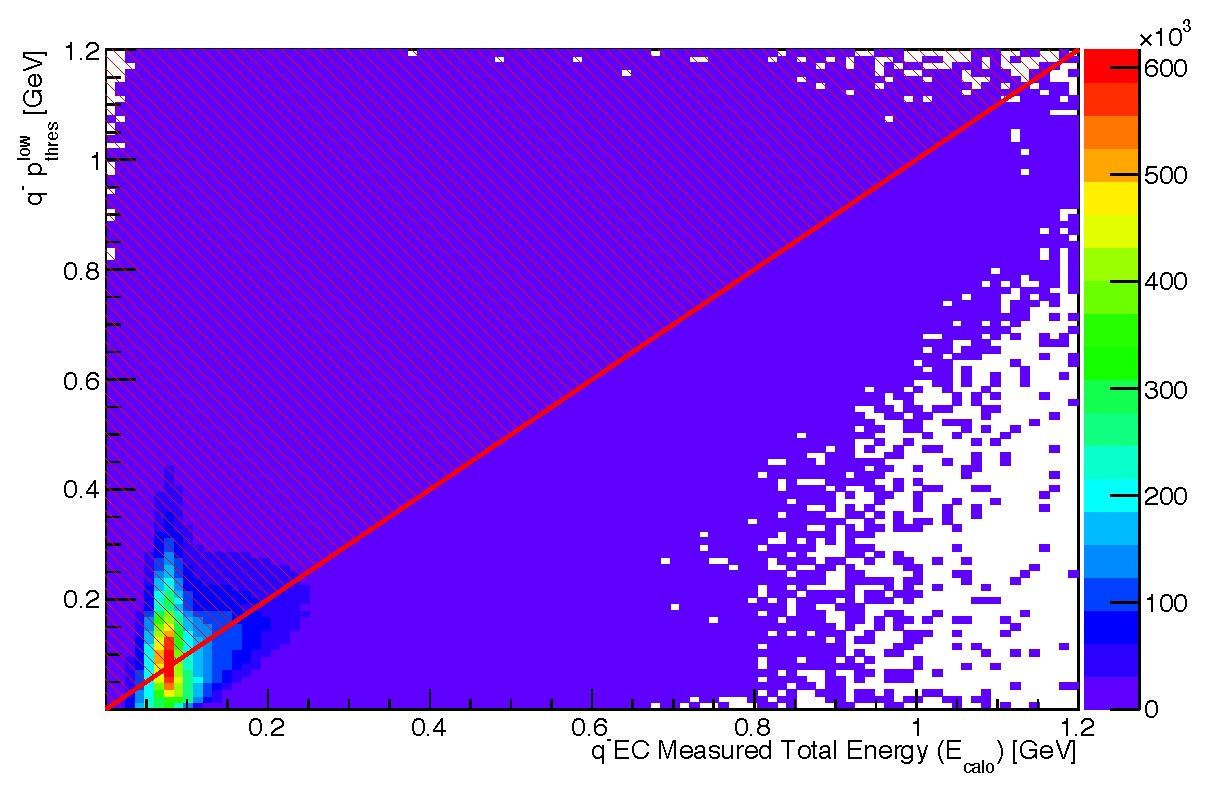
\includegraphics[width=0.8\figwidth]{figures/lepton/Pim_EClow.eps}
				\caption[EC Deposited Energy Comparison to Lower Threshold Track Momentum for q$^-$ Tracks]{\label{fig:islep.pimEClow}Plot of energy deposited measured by EC vs. track momentum p$\mathrm{_{thres}^{low}}$ for negative charged tracks. The red region depicts the cut that would reject events in the g12 lepton EC PID scheme. Image source:~\cite{thesiskunkel}}
\end{center}\end{figure}
			
\begin{figure}\begin{center}
					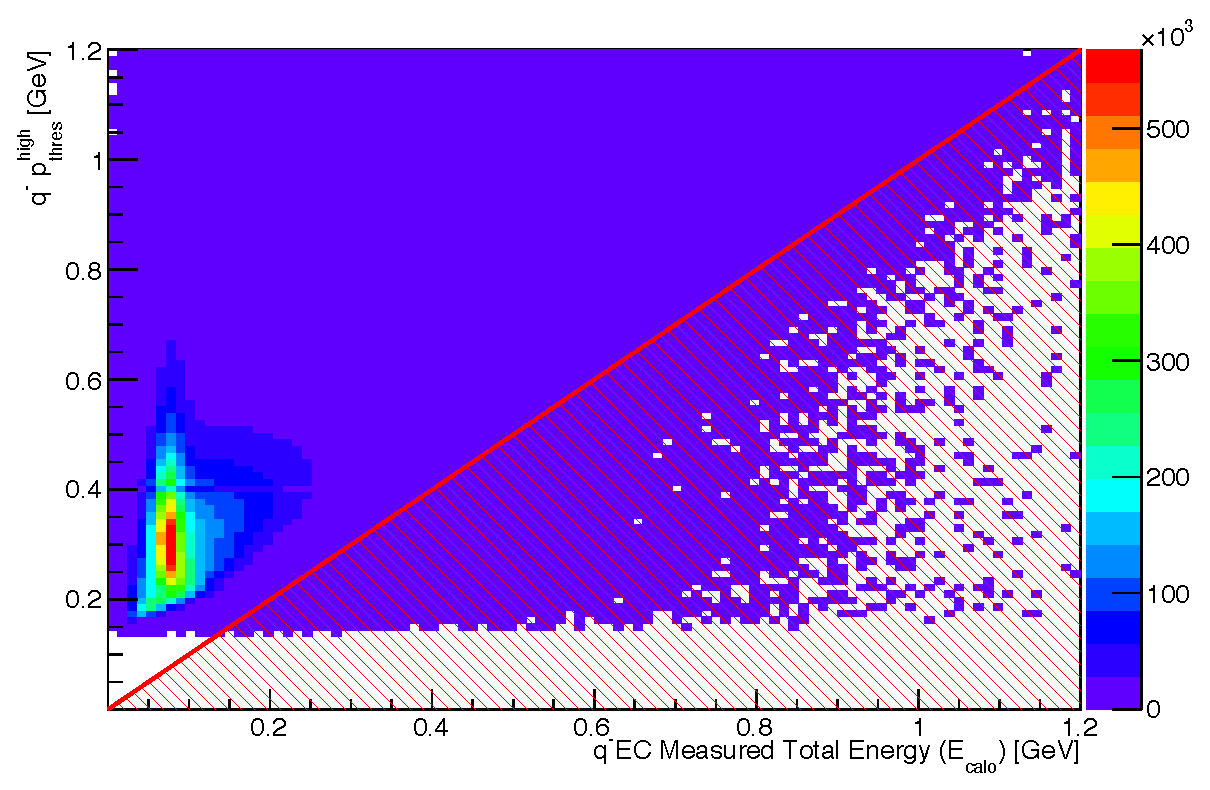
\includegraphics[width=0.8\figwidth]{figures/lepton/Pim_EChigh.eps}
					\caption[EC Deposited Energy Comparison to Upper Threshold Track Momentum for q$^-$ Tracks]{\label{fig:islep.pimEChigh}Plot of energy deposited measured by EC vs. track momentum p$\mathrm{_{thres}^{high}}$ for negative charged tracks. The red region depicts the cut that would reject events in the g12 lepton EC PID scheme. Image source:~\cite{thesiskunkel}}
\end{center}\end{figure}
				
				
\begin{figure}\begin{center}
						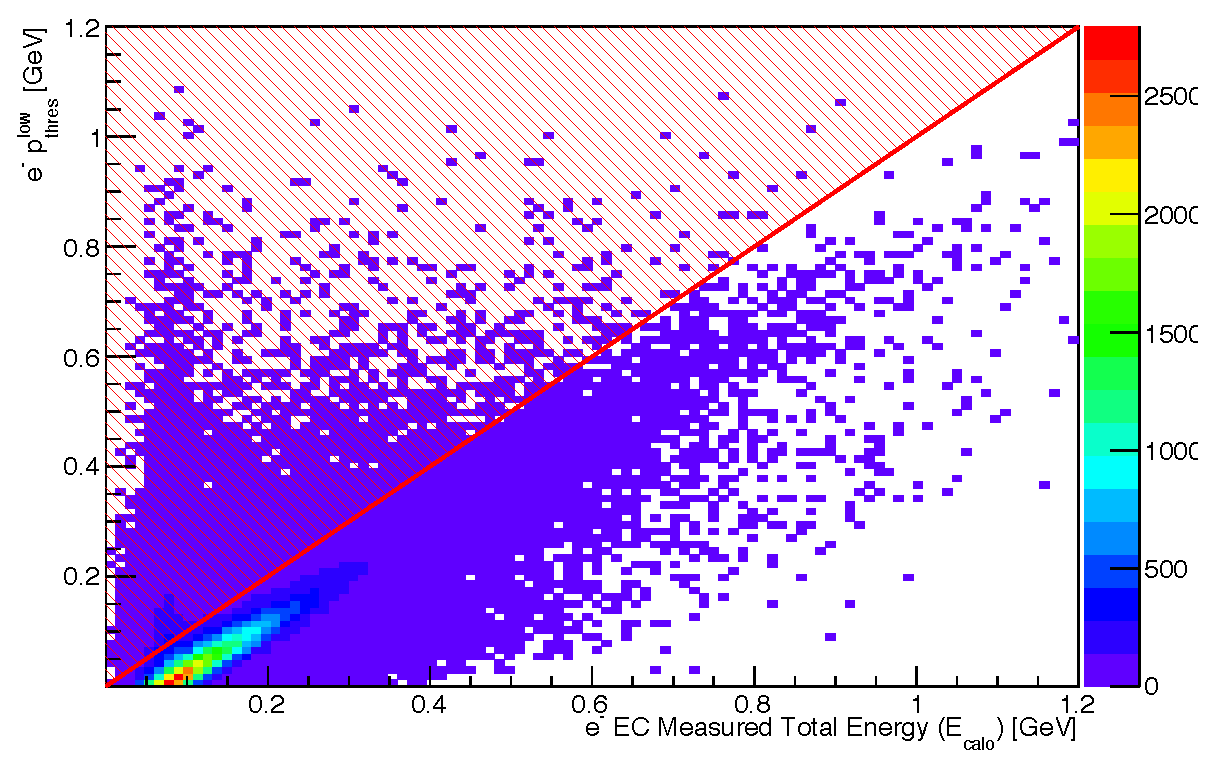
\includegraphics[width=0.8\figwidth]{figures/lepton/Pim_EClowcut.eps}
						\caption[EC Deposited Energy Comparison to Track Momentum for $e^-$ Candidates]{\label{fig:islep.pimEC}Plot of energy deposited measured by EC vs. track momentum p$\mathrm{_{thres}^{low}}$ for electrons from $\pi^0$ events without the g12 lepton EC PID scheme applied. The red region depicts the cut that would reject events in the g12 lepton EC PID scheme. Image source:~\cite{thesiskunkel}}
\end{center}\end{figure}
					
\begin{figure}\begin{center}
							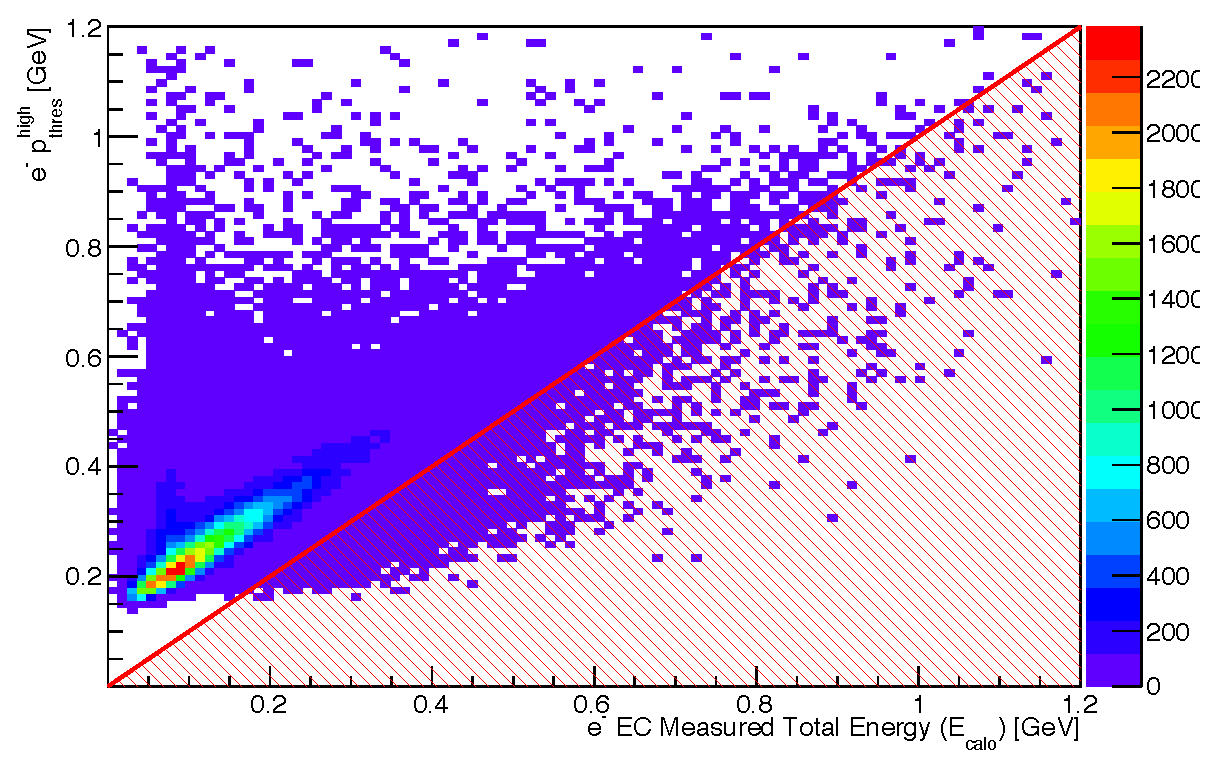
\includegraphics[width=0.8\figwidth]{figures/lepton/Pim_EChighcut.eps}
							\caption[EC Deposited Energy Comparison to Track Momentum for $e^-$ from $\pi^0$ Events]{\label{fig:islep.pimECcut}Plot of energy deposited measured by EC vs. track momentum p$\mathrm{_{thres}^{high}}$ for electrons from $\pi^0$ events without the g12 lepton EC PID scheme applied. The red region depicts the cut that would reject events in the g12 lepton EC PID scheme. Image source:~\cite{thesiskunkel}}
\end{center}\end{figure}
						
Figures~\ref{fig:islep.pipEClow}--\ref{fig:islep.pipECcut} are for positron ($e^+$) PID validation of the g12 EC cuts described in Tab.~\ref{tab:ISLEP_cuts}.
						
\begin{figure}\begin{center}
								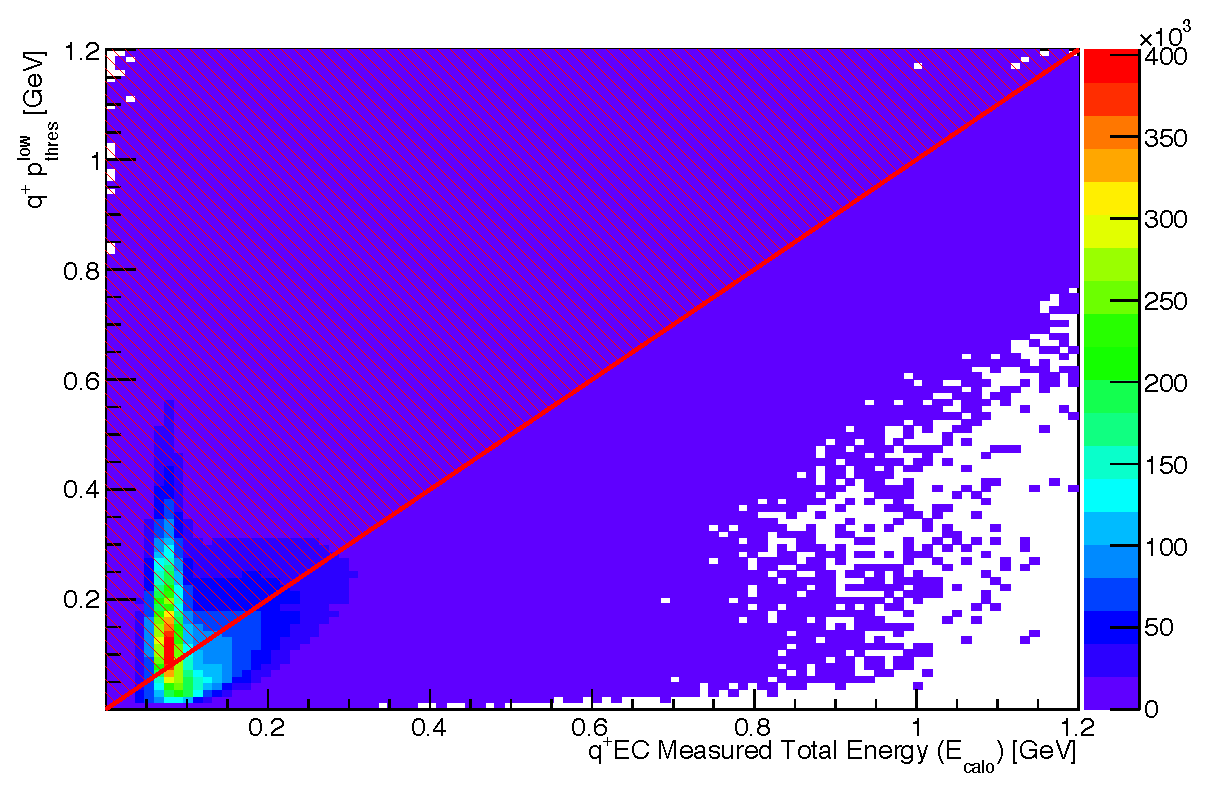
\includegraphics[width=0.8\figwidth]{figures/lepton/Pip_EClow.eps}
								\caption[EC Deposited Energy Comparison to Lower Threshold Track Momentum for q$^+$ Tracks]{\label{fig:islep.pipEClow}Plot of energy deposited measured by EC vs. track momentum p$\mathrm{_{thres}^{low}}$ for positive charged tracks. The red region depicts the cut that would reject events in the g12 lepton EC PID scheme. Image source:~\cite{thesiskunkel}}
\end{center}\end{figure}
							
\begin{figure}\begin{center}
									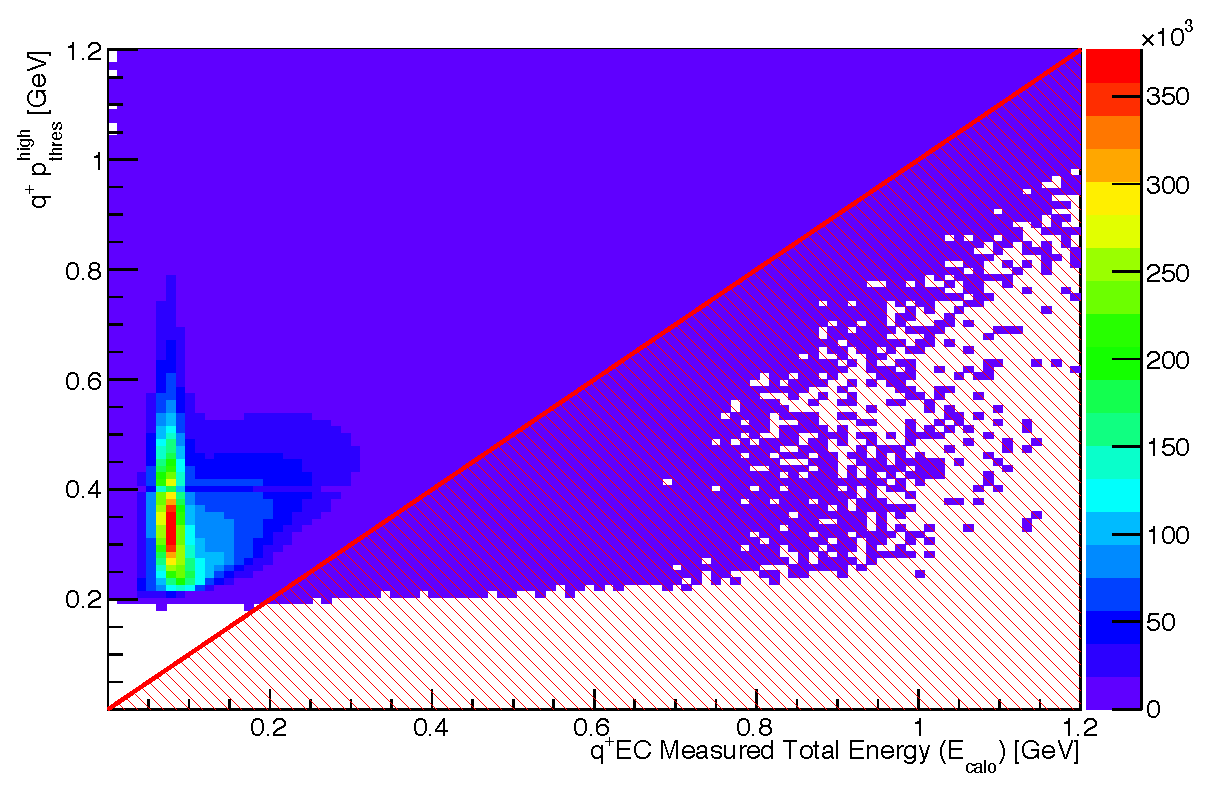
\includegraphics[width=0.8\figwidth]{figures/lepton/Pip_EChigh.eps}
									\caption[EC Deposited Energy Comparison to Upper Threshold Track Momentum for q$^+$ Tracks]{\label{fig:islep.pipEChigh}Plot of energy deposited measured by EC vs. track momentum p$\mathrm{_{thres}^{high}}$ for positive charged tracks. The red region depicts the cut that would reject events in the g12 lepton EC PID scheme. Image source:~\cite{thesiskunkel}}
\end{center}\end{figure}
								
\begin{figure}\begin{center}
										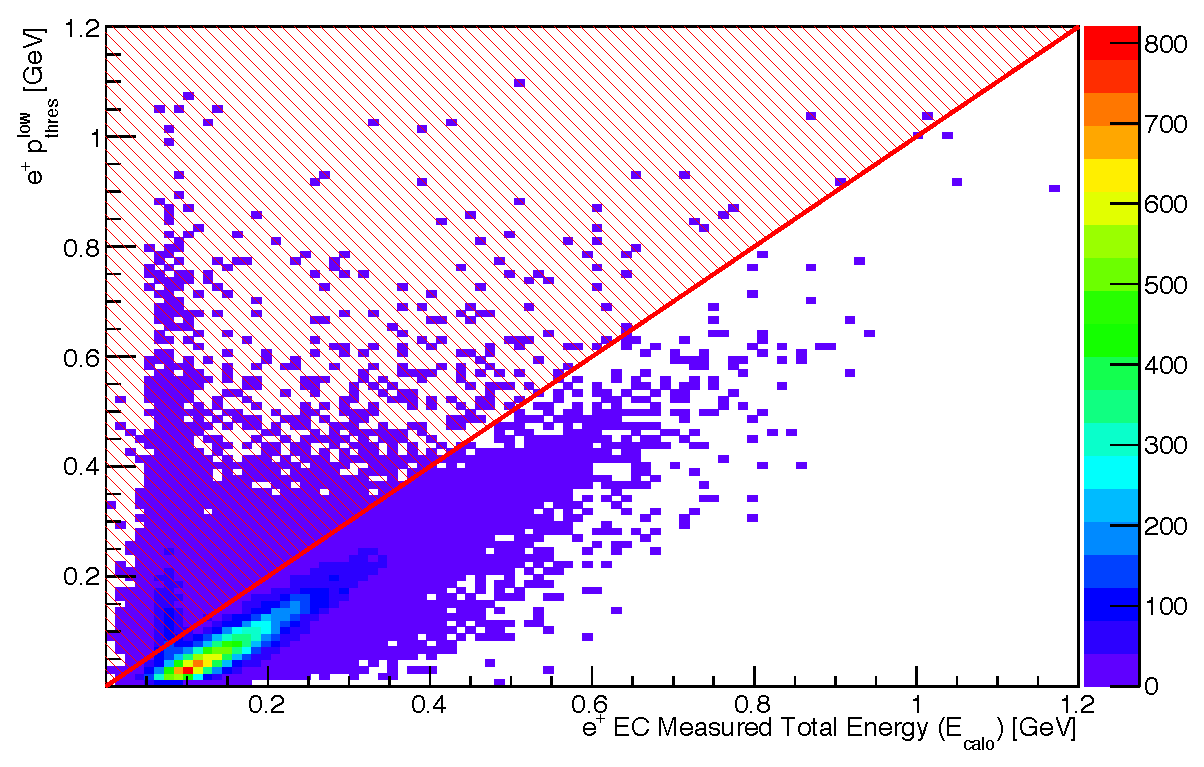
\includegraphics[width=0.8\figwidth]{figures/lepton/Pip_EClowcut.eps}
										\caption[EC Deposited Energy Comparison to Track Momentum for $e^+$ Candidates]{\label{fig:islep.pipEC}Plot of energy deposited measured by EC vs. track momentum p$\mathrm{_{thres}^{low}}$ for positrons from $\pi^0$ events without the g12 lepton EC PID scheme applied. The red region depicts the cut that would reject events in the g12 lepton EC PID scheme. Image source:~\cite{thesiskunkel}}
\end{center}\end{figure}
									
\begin{figure}\begin{center}
											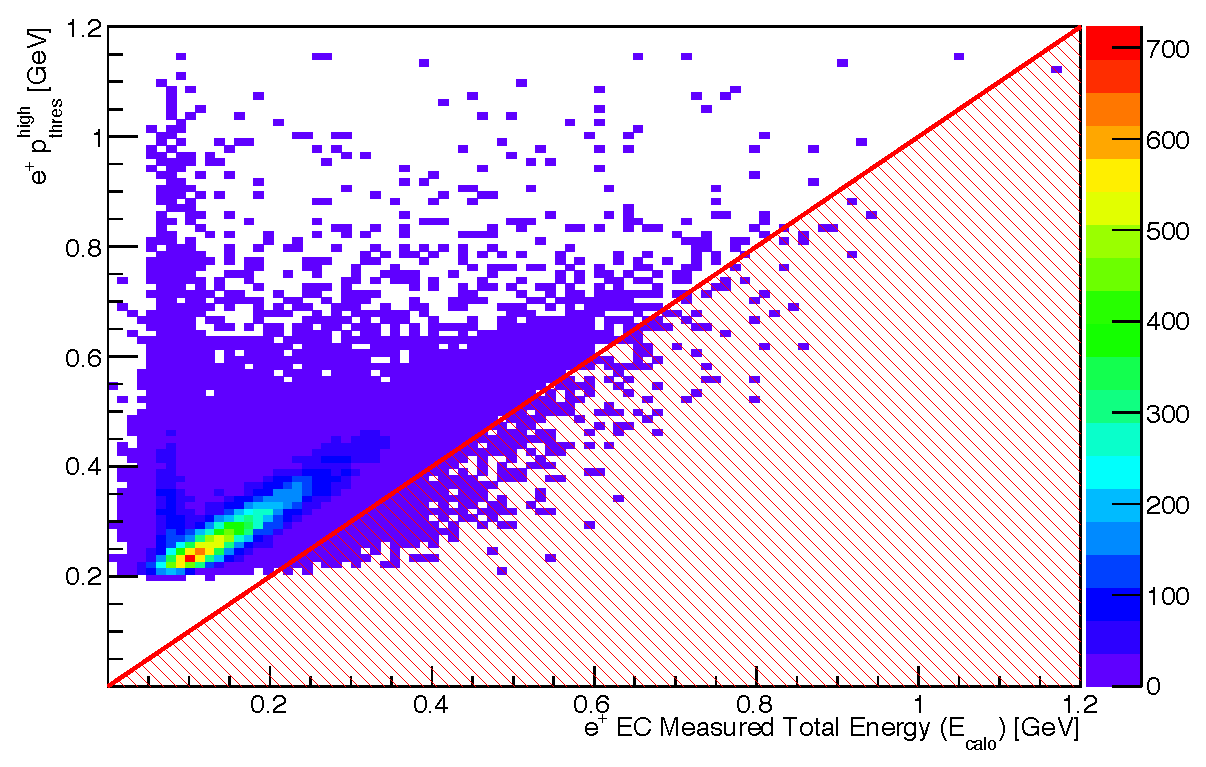
\includegraphics[width=0.8\figwidth]{figures/lepton/Pip_EChighcut.eps}
											\caption[EC Deposited Energy Comparison to Track Momentum for $e^+$ from $\pi^0$ Events]{\label{fig:islep.pipECcut}Plot of energy deposited measured by EC vs. track momentum p$\mathrm{_{thres}^{high}}$ for positrons from $\pi^0$ events without the g12 lepton EC PID scheme applied. The red region depicts the cut that would reject events in the g12 lepton EC PID scheme. Image source:~\cite{thesiskunkel}}
\end{center}\end{figure}																											
\FloatBarrier
\section{\etaPDal \  with CLAS g12}
The CLAS g12 vertex resolution was $\approx 10\,\mathrm{mm}$ (i.e. ten times larger than in the future CLAS12 apparatus) which was not suitable for a sufficient separation between external conversion and Dalitz events. However, the contamination from external conversion was only present in the low $M(\epem)$ mass bins.~\cite{thesisschever}.	Figure~\ref{fig:g12MxP} shows the proton missing mass after reconstruction of  \etaPDal \  events in the CLAS g12 experiment.

\begin{figure}[h!]\begin{center}
		%				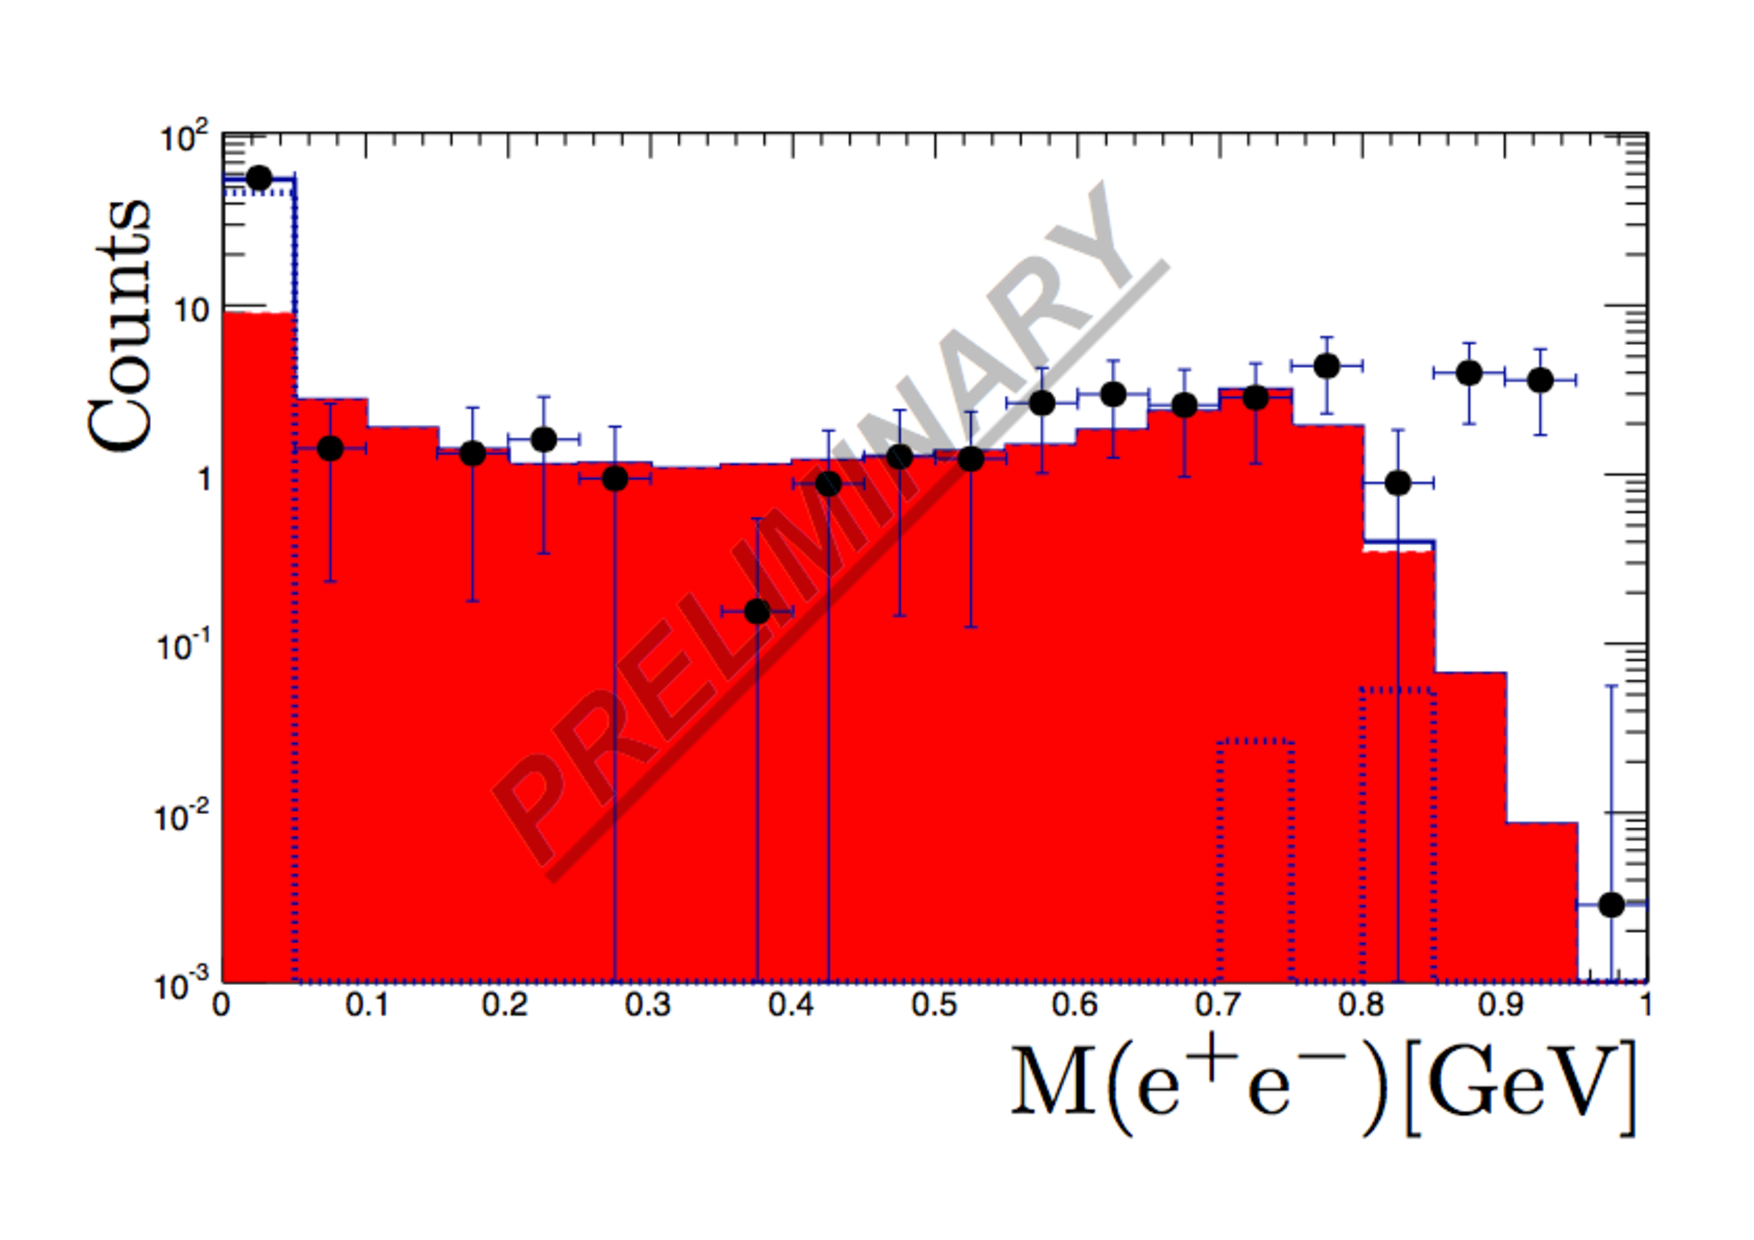
\includegraphics[width=0.8\columnwidth,height=1.0\qfigheight]{\grpath/g12/EpEm_g12.pdf}\label{fig:g12EpEm}
		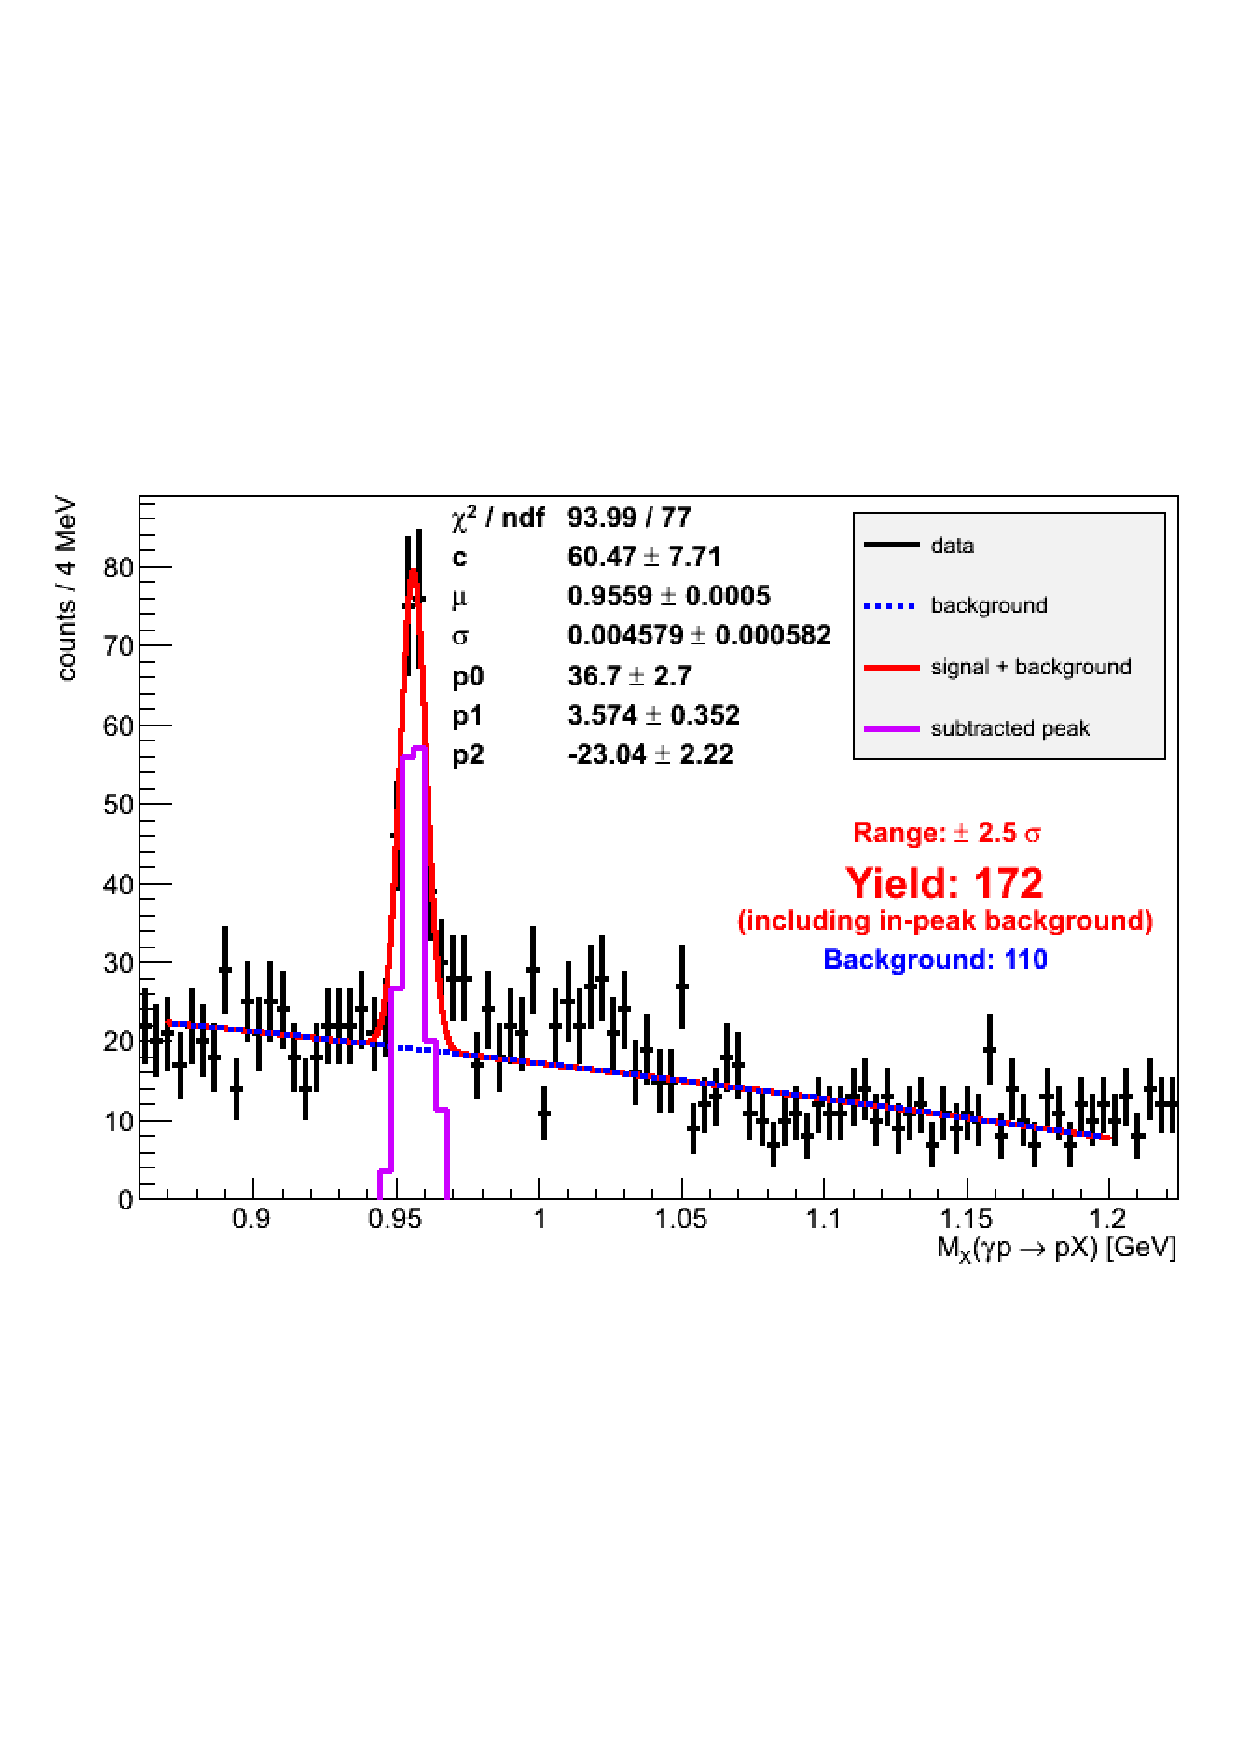
\includegraphics[width=0.8\textwidth]{figures/g12/etaPeeg_mimass.pdf}
		\caption[Counts rates for \etaTP from g12]{\label{fig:g12MxP}Missing mass of the proton for \etaPDal \  from CLAS g12.~\cite{thesisschever} The signal is fitted by a gaussian function whereas the background is fitted by a third order polynomial (blue curve). The sum of both, signal and background, is indicated by the red curve.}
	\end{center}\end{figure}


	
	%I AM NOT SURE HERE. THIS IS PURELY BASED ON MY EXPERIENCE WITH WASA:
	The smooth background is related to Bethe-Heitler and time-like-Compton scattering, which could have been mitigated if the final stated photon from the Dalitz decay would be utilized. The predominant in-peak background contribution is related to the $\eta'\rightarrow \gamma\gamma$ decay.~\cite{thesisschever}.
	The missing mass spectrum in Fig.~\ref{fig:g12MxP} shows the need for a high statistics sample in order to be able to perform a side-band subtraction for the dilepton invariant mass spectrum.
	%direct neutral pion production, which either decay via a dalitz decay or two photons, where one photon produces a dilepton pair via external conversion.
%\section{Signal to Background Separation}
%The CLAS g12 vertex resolution was $\approx 10\,\mathrm{mm}$ (i.e. ten times larger than in the future CLAS12 apparatus) which was not suitable for a sufficient separation between external conversion and Dalitz events. However, the contamination from external conversion was only present in the low $M(\epem)$ mass bins.
%	Using the Qfactor, signal to background separation, technique derived in CLAS~\cite{qfactor}, the total count rate of \etaPDal \ events detected in g12 was $\sim 89$. Figure~\ref{fig:g12figs} depicts the $\etaP$ signal extracted in g12 along with the $M(\epem)$ spectrum from the signal. 
%	\begin{figure}[h!]\begin{center}
%			\subfloat[$\etaP$ Dalitz and conversion spectra from g12][]{ %Feynman diagram of $\etaP$ two photon decay
%				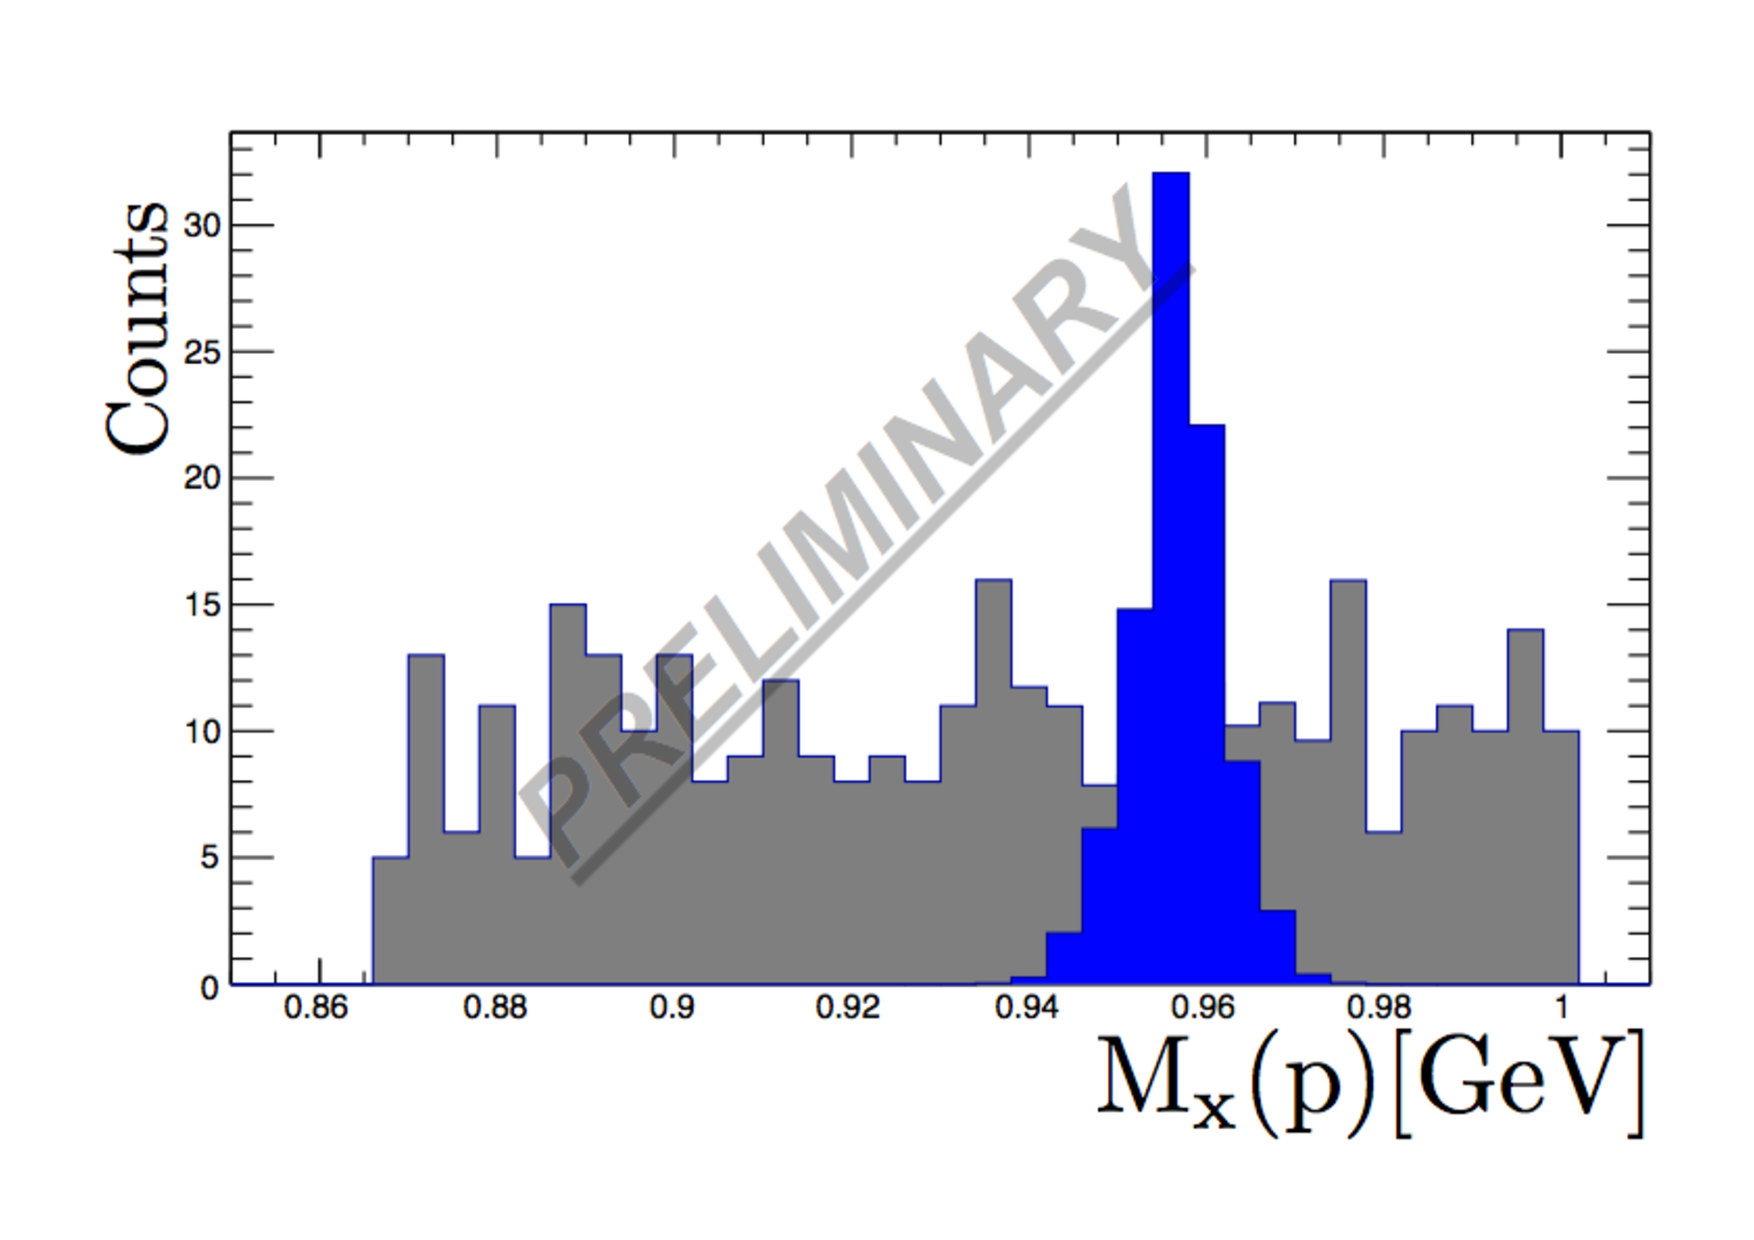
\includegraphics[width=0.8\columnwidth,height=1.0\qfigheight]{\grpath/g12/MxP_g12.pdf}\label{fig:g12MxP}
%			}
%			\\
%			\subfloat[$\phi$ Dalitz and conversion spectra from g12][]{ %Feynman diagram of $\etaP$ Dalitz decay
%				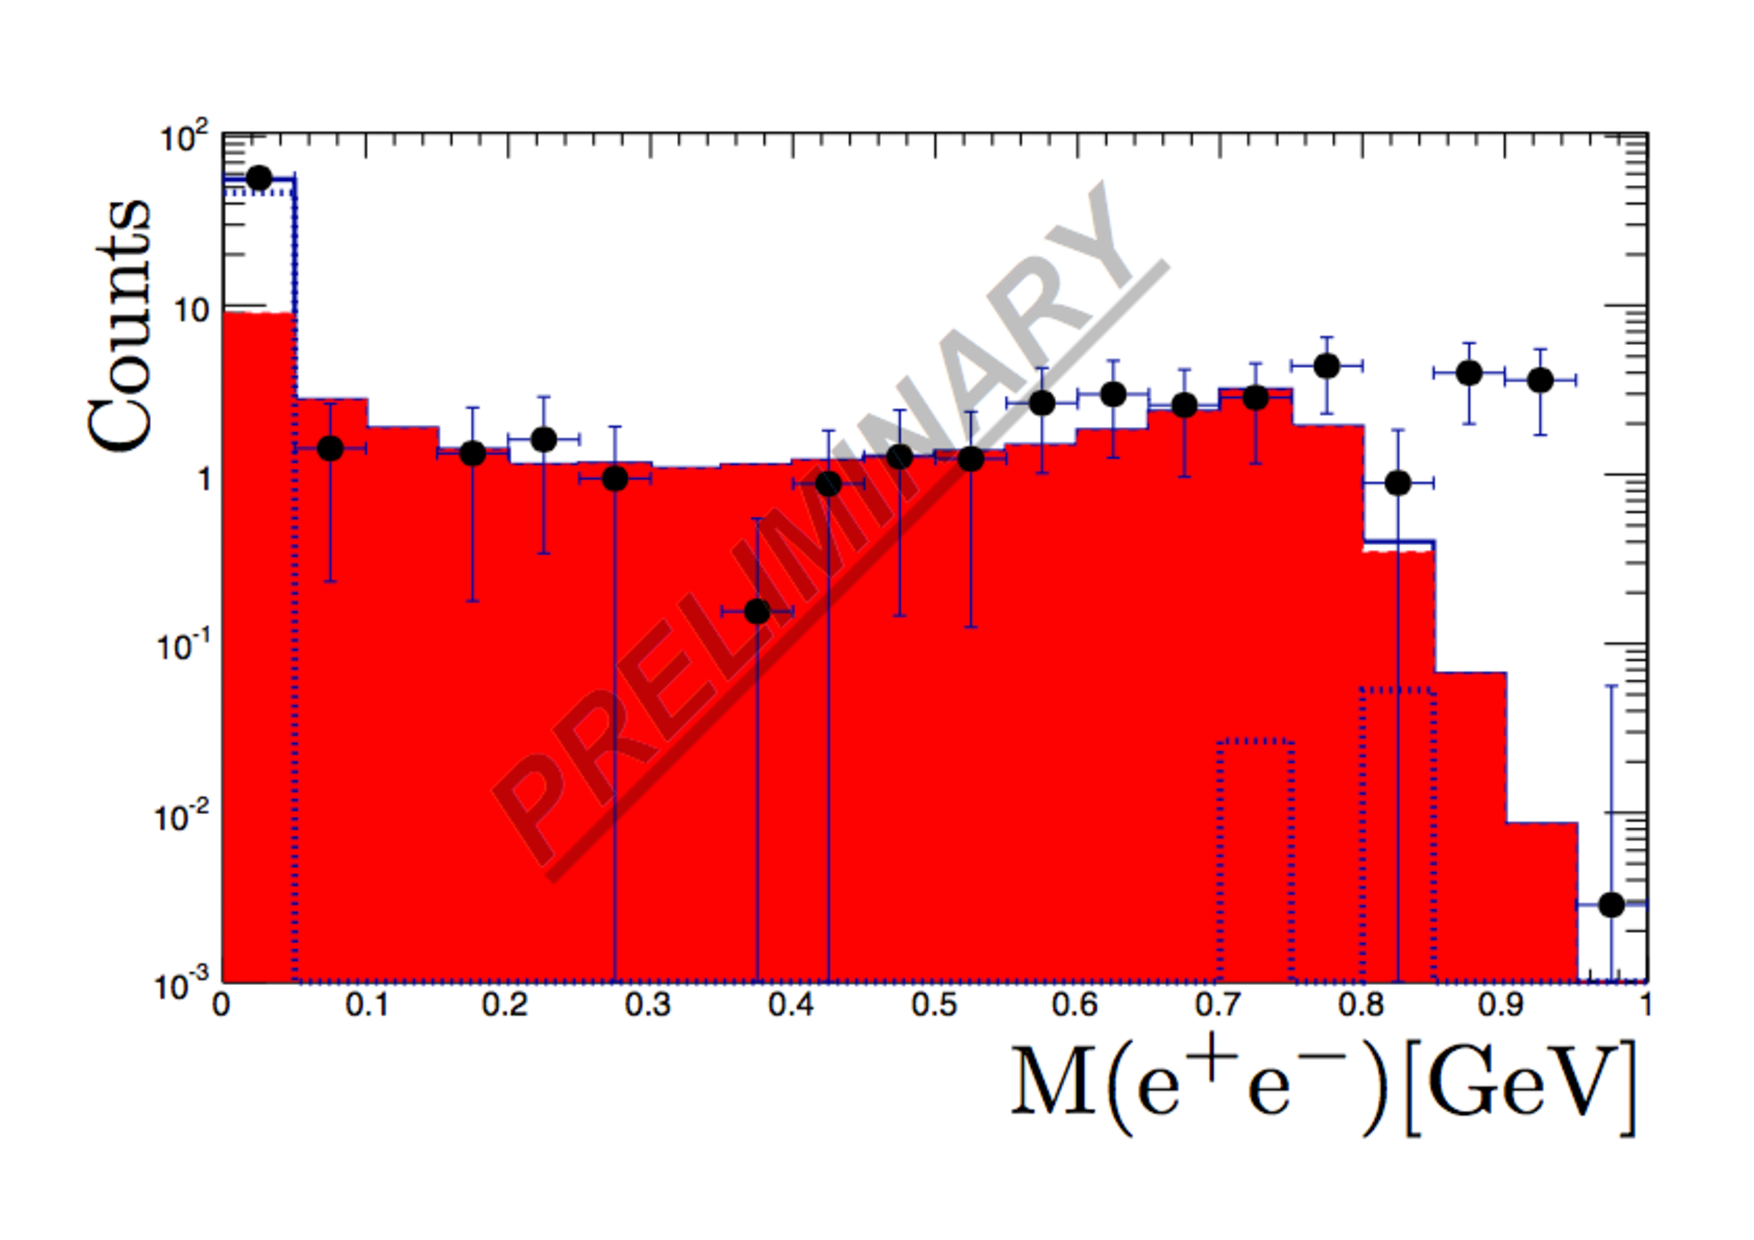
\includegraphics[width=0.8\columnwidth,height=1.0\qfigheight]{\grpath/g12/EpEm_g12.pdf}\label{fig:g12EpEm}
%			}
%			\caption[Counts rates for \etaTP from g12]{\label{fig:g12figs}~\subref{fig:g12MxP} Missing mass off of the proton for \etaPDal \  from CLAS g12. Q-factor weighted(Blue), Background (Grey). ~\subref{fig:g12EpEm} Invariant mass spectrum of \epemT \ under the blue curve in~\subref{fig:g12MxP}. Total counts in 29 days $\sim$ 89.}
%		\end{center}\end{figure}
%		\FloatBarrier 	
%		As seen in Fig.~\ref{fig:g12figs} the current CLAS results suffer from insufficient statistics. Therefore, we propose to repeat the \etaPDal \  measurement with CLAS12.
		\FloatBarrier